\documentclass[12pt, a4paper]{article}
\usepackage[utf8]{inputenc}
\usepackage[T2A]{fontenc}
\usepackage[russian]{babel}
\usepackage[oglav,spisok,boldsect,eqwhole,figwhole,hyperref,hyperprint,remarks,greekit]{fn2kursstyle}


\usepackage{subfig}
\usepackage{amsfonts}
\usepackage{mathtools}
\usepackage{enumitem}
\usepackage{pifont}
\usepackage{changepage}
\usepackage{multirow}
\usepackage{supertabular}
\usepackage{multicol}
\usepackage{scalerel}
\usepackage{graphicx}

\usepackage{colortbl}
\usepackage{nicematrix}
\usepackage{stackengine}


\graphicspath{
	{./style/}
	{./illustr/}
	{./illustr/domain_rectangle_dirichlet_only/}
	{./illustr/domain_4/}
	{./illustr/domain_1_1/}
}

\frenchspacing
\sloppy
\counterwithout{equation}{section}
\counterwithout{figure}{section}
\newenvironment{comment}{}{}


% Параметры титульного листа
\title{Поиск потенциала электрического поля между заряженными пластинами}
\author{А.\,Д.~Егоров}
\supervisor{К.\,Е.~Казаков}
\group{ФН2-62Б}
\date{2023}

% Переопределение команды \vec, чтобы векторы печатались полужирным курсивом
\renewcommand{\vec}[1]{\text{\mathversion{bold}${#1}$}}%{\bi{#1}}

\renewcommand{\phi}{\varphi}
\newcommand\Tau{\scalerel*{\tau}{T}}

\newcommand\thh[1]{\text{\mathversion{bold}${#1}$}}
\newcommand\xrowht[2][0]{\addstackgap[.5\dimexpr#2\relax]{\vphantom{#1}}}
%Переопределение команды нумерации перечней: точки заменяются на скобки
%\renewcommand{\labelenumi}{\theenumi)}
\renewcommand{\labelenumii}{\arabic{enumi}.\arabic{enumii}}
\renewcommand{\labelenumiii}{\arabic{enumi}.\arabic{enumii}.\arabic{enumiii}}
\renewcommand{\labelenumiv}{\arabic{enumi}.\arabic{enumii}.\arabic{enumiii}.\arabic{enumiv}}



\begin{document}
	
	\maketitle	
	\tableofcontents
	\newpage
	
	\section-{Введение}
		Задача по вычислению потенциала электрического поля является задачей раздела электростатики. Она возникает при вычислении электростатического поля в различных конденсаторах. Ее решение сводится к решению уравнения Пуассона или его частного случая --- уравнения Лапласа. Данные уравнения появляются и при решении ряда задач из других сфер: аэродинамики, гидродинамики, механики сплошных сред. Так что методы примененные в данной работе, могут быть применены и к другим задачам, что показывает актуальность данной проблемы.
		
	
	\section {Постановка задачи}
		
		Найти потенциал электрического поля между двумя бесконечными пластинами, профиль одной из которых плоский, а профиль другой описывается некоторой периодической функцией. Значения потенциала на пластинах заданы и константны.		
		
		
	%\newpage
	\section{Обзор задачи}
	
		
		\subsection{Физическая составляющая задачи}
			\looser{-0.02}{Для постоянного электрического (электростатического) поля уравнения Максвелла имеют вид}
			\begin{equation}
				\mathrm{div} \vec{\mathrm{E}} = 4 \pi \rho,
				\label{div_E}
			\end{equation}
			\begin{equation}
				\mathrm{rot} \vec{\mathrm{E}} = 0,
				\label{rot_E}
			\end{equation}
			где $\rho$ --- объемная плотность внешних зарядов. Электрическое поле $\vec{\mathrm{E}}$ выражается через только скалярный потенциал соотношением
			\begin{equation}
				\vec{\mathrm{E}} = -\mathrm{grad} \varphi,
				\label{E_grad_phi}
			\end{equation}
			подставляя (\refeq{E_grad_phi}) в (\refeq{div_E}), получим уравнение, которому удовлетворяет потенциал постоянного электрического поля:
			\begin{equation}
				\Delta \varphi = - 4 \pi \rho.
				\label{Pois_eq}
			\end{equation}
			Уравнение (\refeq{Pois_eq}) есть уравнение Пуассона. При $\rho = 0$, т.е. при отсутствии внешних сил, потенциал удовлетворяет уравнению Лапласа \cite{Landau}
			\begin{equation}
				\Delta \phi = 0.
				\label{Laplace_eq}
			\end{equation}
			
		\subsection{Математическая постановка задачи}
			
			Из условия поставленной задачи известно, что внешних сил нет, следовательно, потенциал электростатического поля должен удовлетворять уравнению (\refeq{Laplace_eq}). Через функцию $w(x)$ зададим профиль искривленной пластины, $w(x)$  --- некоторая периодическая функция с периодом $T$, т.е. $w(x) = w(x + T)$. Пусть плоская пластина находится над искривленной на уровне $y_a$. Значение потенциала на пластинах заданы и константны, обозначим значение на верхней (плоской) пластине как $\phi_a$, на нижней (искривленной) --- $\phi_w$. Так как профиль профиль задан периодической функцией, следовательно необходимо использовать условие равенства потенциалов в точках $x$ и $x + T$, т.е. $\phi (x, y) = \phi (x + T, y)$.
			
			Из этих условий составим систему, которую требуется решить: 		
			\begin{equation}
				\begin{cases}
					\Delta \phi (x, y)  = 0, \\
					\phi (x, y_a) = \phi_a, \\
					\phi (x, w(x)) = \phi_w, \\
					\phi (x, y) = \phi (x + T, y).\\
					
				\end{cases}
			\end{equation}
			\begin{figure*}[!h]
				\centering
				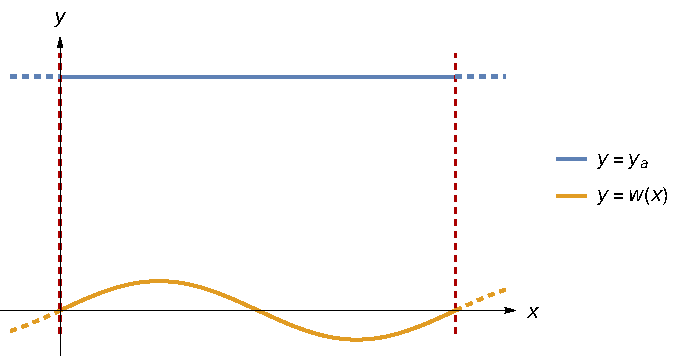
\includegraphics[width=1\textwidth]{illustr.pdf}
				\caption{Иллюстрация области, в которой будет решаться задача}
				\label{fig:illustr_1}
			\end{figure*}
	
	\newpage
	\section{Решение двумерного уравнения Лапласа}
		
		
		\subsection{Аппроксимация уравнения Лапласа}
		
			Рассмотрим уравнение Лапласа в двумерной области $\Omega \subset \mathbb{R}^2$
			\begin{equation*}
				\begin{cases}
					- \Delta u  = 0 \ \  \text{в}\ \  \Omega, \\
					u = g \ \ \text{на}\ \  \Gamma_D,
				\end{cases}			
			\end{equation*}
			где $\Gamma_D$ --- часть границы области, на которой заданы граничные условия первого рода, $\Gamma_D = \partial \Omega,$  $\Gamma_D \ne \emptyset$. 
			
			Опираясь на сведения из источника \cite{Galanin}, представим решение задачи в виде $u = u_0 + u_g$, где функция $u_0$ обращается в ноль на границе $\Gamma_D$ а $u_g$ --- некоторая, произвольная, но наперед заданная функция, значения которой совпадают с $g$ на границе области, $u_g |_{\Gamma_D} = g$.
			
			И переходим к следующей задаче с однородными граничными условиями первого рода на $\Gamma_D$ относительно функции $u_0$:
			\begin{equation*}
			\begin{cases}
				- \Delta u  = \Delta u_g \ \  \text{в}\ \  \Omega, \\
				u_0 = 0 \ \ \text{на}\ \  \Gamma_D.
			\end{cases}			
			\end{equation*}
			
			\looser{0.0}{Запишем слабую постановку задачи для определения $u_0$, способом описанным в разделе \textbf{16.3.1}} источника \cite{Galanin}: необходимо определить $u_0 \in V_D$, такое, что 
			\begin{equation*}
				\int_{\Omega} \nabla u_0 \cdot \nabla v \, d\Omega = 
				- \int_{\Omega} \nabla u_g \cdot \nabla v \, d\Omega, \quad v \in V_D,
			\end{equation*}			
			\looser{-0.014}{где пространство $V_D$ состоит из функций, имеющих суммируемые с квадратом первые производные и обращающихся в ноль на части $\Gamma_D$ границы расчетной области:}
			\begin{equation*}
				V_D = \left\{ v \in V: \ v |_{\Gamma_D} = 0 \right\},
			\end{equation*}
			а пространство $V$ состоит из произвольных заданных в $\Omega$ функций, имеющих суммируемые с квадратом первые производные.
			
			Для аппроксимации задачи с помощью МКЭ рассмотрим конечномерное пространство $V_h$, аппроксимирующее пространство $V$ и пространство 
			$V_{D,h} = V_h \cap V_D(\Omega)$, элементы которого приближают элементы пространства $V_D$. 
			
			Пусть функция $u_{g,h} \in V_h $ представляет собой аппроксимацию функции $u_g$, задающей граничное условие первого рода. В качестве функции $u_{g,h}$. 
			
			Тогда конечномерная задача примет вид: 
			%определить $u_{0,h} \in V_{D,h}$, такую, что
			
			\begin{equation*}
				\int_{\Omega} \nabla u_{0,h} \cdot \nabla v_{h} \, d\Omega = 
				- \int_{\Omega} \nabla u_{g,h} \cdot \nabla v_{h} \, d\Omega, \quad v_{h} \in V_{D,h},
			\end{equation*}
			
			Пусть $\phi_i$, \ i = $\overline{1, N},$ --- базис в пространстве $V_h$, причем часть функций $\phi_i$ с номерами $i \in I$ образуют базис в пространстве $V_{D,h}$, т.е. обращаются в ноль на границе $\Gamma_D$. Количество таких индексов будем считать равным $M = |I| < N,\ |I| > 1$.
			
			Тогда последнее уравнение будет эквивалентно
			\begin{equation*}
				\int_{\Omega} \nabla u_{0,h} \cdot \nabla \phi_{i} \, d\Omega = 
				- \int_{\Omega} \nabla u_{g,h} \cdot \nabla \phi_{i} \, d\Omega, \quad i \in I.
			\end{equation*}
			
			Представляя неизвестное решение в виде линейной комбинации базисных функций:
			\begin{equation*}
				u_{0,h} = \sum_{i \in I} u_{0,h,i} \phi_i, \quad 
				u_{g,h} = \sum_{i = 1}^{N} u_{g,h,i} \phi_i, 
			\end{equation*}
			\looser{-0.0}{окончательно получим СЛАУ для определения неизвестных коэффициентов 
			$U_h = \left\{ u_{0, h, i}\right\}$:}
			\begin{equation*}
				A u_{0,h} = b,
			\end{equation*}
			где $A = A_{M \times M}$ --- матрица жесткости, $b = b_{M \times 1}$,
			\begin{equation}
				A_{ij} = \int_{\Omega} \nabla \phi_i \cdot \nabla \phi_j \, d\Omega,
				\quad i, j\in I,
				\label{A_stiff_first}				
			\end{equation}
			\begin{equation}
				b_i = - \sum_{j=1}^{N} u_{g,h, j} \int_{\Omega} \nabla \phi_i  \cdot \nabla \phi_j \, d\Omega, \quad i \in I.
				\label{b_stiff_first}
			\end{equation}
			
			
		\subsection{Метод конечных элементов на треугольной сетке}
			
			\subsubsection{Триангуляция области}
			
				\looser{-0.012}{Зададим в нашей области $\Omega$ правильную триангуляцию $\Tau$, т.~е. такое разбиение области $\Omega$ на треугольные ячейки, что любые два треугольника имеют либо общее ребро, либо общую вершину, либо пустое пересечение.} Таким образом, 
				\begin{equation*}
					\Omega = \underset{T \in \Tau}{\bigcup}T.
				\end{equation*}
				
				Каждый треугольник $T$ при этом задается набором трех своих узлов $P_k$ с координатами $P_k = (x_k, y_k)$. Будем считать, что узлы треугольника обходятся в положительном направлении (против хода часовой стрелки).
				
				Рассмотрим простейший случай: выберем базисные функции $\phi_k$ такие, что $\phi_k$ --- кусочно-линейная функция, принимающая значение единица в узле $P_k$ и ноль во всех остальных узлах, в пределах одного треугольника она продолжена линейно.
				
				В силу аддитивности интеграла относительно области интегрирования  формулы (\refeq{A_stiff_first}) и (\refeq{b_stiff_first}) могут быть записаны в виде			
				\begin{equation}
					A_{ij} = \sum_{T \in \Tau}\int_{T} \nabla \phi_i \cdot \nabla \phi_j \, d\Omega,
					\quad i, j\in I,
					\label{A_stiff_second}				
				\end{equation}
				\begin{equation}
					b_i = - \sum_{j=1}^{N} u_{g,h, j} \sum_{T \in \Tau} \int_{T} \nabla \phi_i  \cdot \nabla \phi_j \, d\Omega, \quad i \in I.
					\label{b_stiff_second}
				\end{equation}
				
				Таким образом, задача вычисления интегралов для коэффициентов матрицы жесткости задачи и ее правой части сводится к задаче вычисления тех же интегралов по отдельным треугольникам.
				
				
				Рассмотрим один из треугольников $T$ триангуляции $\Tau$. Будем считать, что его вершины имеют координаты  $P_i = (x_i, y_i), \ i=\overline{1,3}$. Пусть $\phi_i, \ i=\overline{1,3}$, --- базисные функции соответствующие этим вершинам и данному треугольнику. Таким образом 
				\begin{equation*}
					\phi_i(x_j, y_j) = \delta_{ij}, \ i,j = 1,2,3.
				\end{equation*}
				Функции $\phi_i$ являются линейными в пределах $T$ и имеют следующий вид
				\begin{equation}
					\phi_i(x,y) = 
					\dfrac{
						\det{
							\begin{pmatrix}
								1 & x & y \\
								1 & x_{i+1} & y_{i+1} \\
								1 & x_{i+2} & y_{i+2} \\							
							 \end{pmatrix}
						 }
					}{
					\det{
						\begin{pmatrix}
							1 & x_{i} & y_{i} \\
							1 & x_{i+1} & y_{i+1} \\
							1 & x_{i+2} & y_{i+2} \\							
						\end{pmatrix}
						}
					}, \quad i = 1,2,3,
					\label{basis_fun_phi}
				\end{equation}
				где для удобства обозначения считается, что $P_4 = P_1, \ x_4 = x_1, \ y_4 = y_1, $ аналогично индекс 5 идентичен индексу 2.
				
				Из формулы (\refeq{basis_fun_phi}) получаем следующие соотношения:
				\begin{equation*}
					\nabla \phi_{i}(x,y) = \dfrac{1}{2 |T|} 
					\begin{pmatrix}
						y_{i+1} - y_{i+2} \\
						x_{i+2} - x_{i+1} \\
					\end{pmatrix},
				\end{equation*}
				где $|T|$ --- площадь треугольника $T$, такая, что
				\begin{equation*}
					|T| = \dfrac{1}{2} 
					det{
						\begin{pmatrix}
							x_2 - x_1 & x_3 - x_1 \\
							y_2 - y_1 & y_3 - y_1 \\
						\end{pmatrix}				
					}.
				\end{equation*}
				
				В результате получаем следующее выражение для матрицы жесткости конечного элемента $T$:
				\begin{eqnarray}
					A_{T,ij} = \int_{T} \nabla \phi_i \cdot \nabla \phi_j \, d\Omega
					= \dfrac{|T|}{(2|T|)^2} 
					\begin{pmatrix}
						y_{i+1} - y_{i+2}\\
						x_{i+2} - x_{i+1}\\
					\end{pmatrix}^T
					\begin{pmatrix}
						y_{j+1} - y_{j+2}\\
						x_{j+2} - x_{j+1}\\
					\end{pmatrix},
					\quad i,j=1,2,3.
					\label{A_stiff_in_T}
				\end{eqnarray}
				
			\subsubsection{Сборка глобальной матрицы жесткости}
				
				В предыдущем пункте было рассмотрено, как составляется матрица жесткости для одного элемента $T$ триангуляции $\Tau$. Основываясь на формулах (\refeq{A_stiff_second}, \refeq{b_stiff_second}, \refeq{A_stiff_in_T}) для каждого элемента $T$ триангуляции $\Tau$  имеем: 
				\begin{itemize}
					\item $A_T$ --- симметричная матрица размером $3 \times 3$,
					\item $b_T$ --- вектор правой части, состоящий из 3, компонент,
					\item $u_T$ --- вектор неизвестных, состоящий из 3 компонент.
				\end{itemize}
				%\vspace*{-6mm}
				%\begin{table}[!h]
				%	\begin{center}
				%%			\hline
				%			\multicolumn{2}{|c|}{ для каждого элемента $T$ триангуляции $\Tau$} \\
				%			\hline
				%			$A_T$ & симметричная матрица размером $3 \times 3$,\\
				%			\hline
				%			$b_T$ & вектор правой части, состоящий из 3, компонент,\\
				%			\hline
				%			$u_T$ & вектор неизвестных, состоящий из 3 компонент.\\
				%			\hline
				%		\end{tabular}
				%	\end{center}
				%\end{table}
				%\vspace*{-6mm}
								
				\noindent
				Для решения задачи необходимо составить полную систему $Au = b$, где $A$ --- матрица жесткости размером $N \times N$, $b$ --- вектор правой части длины $N$, $u$ --- вектор неизвестных длины $N$, $N$ --- количество узлов триангуляции $\Tau$, для этого нужно собрать все локальные матрицы жесткости $A_T$, т.~е. учесть вклад каждого конечного элемента.
				
				Проиллюстрируем эту процедуру на примере. У нас есть треугольник $T$, составленный из узлов $P_1 = (x_1, y_1), \ P_3 = (x_3, y_3), \ P_5 = (x_5, y_5)$ (номера узлов взяты из глобальной нумерации), для него были получены следующая матрица жесткости $A_T$ и вектор правой части $b_T$
				\begin{equation*}
					A_T = \begin{pmatrix}
						\phantom{-}1.3 & -0.5 & \phantom{-}7 \\
						-0.5 & -0.45 & \phantom{-}0.3 \\
						\phantom{-}7 & \phantom{-}0.3 & \phantom{-}2.1 \\
					\end{pmatrix},
					\quad
					b_T = \begin{pmatrix}
						2 \\
						2.1 \\
						1 \\
					\end{pmatrix}.
				\end{equation*}
				Допустим, что полная система состоит из 7 узлов. Тогда мы расширяем матрицу $A_T$ до размера $7 \times 7$, добавляя нулевые строки и столбцы на место отсутствующих узлов, аналогично для вектора 
				$b_T$. Таким образом получаем следующие матрицу и вектор правой части
				\begin{equation*}
					\widehat A_T = 
					\begin{pmatrix}
						\phantom{-}1.3 & 0 & -0.5         & 0 & \phantom{-}7   & 0 & 0\\
						  \phantom{-}0 & 0 & \phantom{-}0 & 0 & \phantom{-}0   & 0 & 0\\
						          -0.5 & 0 & -0.45        & 0 & \phantom{-}0.3 & 0 & 0\\
						  \phantom{-}0 & 0 & \phantom{-}0 & 0 & \phantom{-}0   & 0 & 0\\
					   	  \phantom{-}7 & 0 &\phantom{-}0.3& 0 & \phantom{-}2.1 & 0 & 0\\
						  \phantom{-}0 & 0 & \phantom{-}0 & 0 & \phantom{-}0   & 0 & 0\\
						  \phantom{-}0 & 0 & \phantom{-}0 & 0 & \phantom{-}0   & 0 & 0\\
					\end{pmatrix},
					\quad
					\widehat{b}_T = \begin{pmatrix}
						2 \\
						0 \\
						2.1 \\
						0 \\
						1 \\
						0 \\
						0 \\
					\end{pmatrix}.
				\end{equation*}
				
				Тогда для полной системы матрица $A$ и вектор правой правой части $b$ имеют следующий вид
				\begin{equation*}
					A = \sum_{T \in \Tau} \widehat{A}_T, \quad 
					b = \sum_{T \in \Tau} \widehat{b}_T.
				\end{equation*}
				
			\subsubsection{Применение граничных условий первого рода}
			
				Полную систему уравнений $A u = b$ можно записать в виде 
				\begin{equation}
					\sum_{j = 1}^{N} a_{ij} u_{j} = b_i, \quad i = \overline{1,N},
					\label{sys_in_index}
				\end{equation}
				где $a_{ij}$ --- компоненты матрицы $A$, а $b_{j}$, и $u_{j}$ --- компоненты вектора правой части $b$ и вектора неизвестных $u$ соответственно. Значения решения в узлах, принадлежащих границе $\Gamma_D$ известны и равны $u_k = g(P_k), \forall k \in K$, где $K$ --- множество индексов узлов принадлежащих границе $\Gamma_D$. Тогда уравнения (\refeq{sys_in_index}) могут быть перезаписаны следующим образом
				\begin{equation}
					\sum_{j \in I} a_{ij} u_{j} = 
					b_i - \sum_{k \in K} a_{ij} g(P_j), 
					\quad i \in I,
					\label{sys_in_index_plus_dirichlet}
				\end{equation}
				где, как было указано выше, $I$ --- множество индексов узлов, лежащих внутри области, $|I| + |K| = N$. Что приводит к уменьшению размера  матрицы $A$ от $N \times N$ до $M \times M$, по средствам удаления строк и столбцов с номерами $k \in K$ \cite{Galanin}.
				
			\subsubsection{Применение периодических граничных условий}
				
				В поставленной задаче помимо условий первого рода дополнительно наложены условия периодичности на левой и правой границах.
				Обозначим множество индексов узлов, принадлежащих данной данной части границы, как $PB$. Это множество такое, что
				\begin{equation*}
				 	PB = PB_l \cup PB_r,
				\end{equation*}
				\looser{-0.01}{где $PB_l$ --- множество индексов узлов принадлежащих левой границе, $PB_r$ --- множество индексов узлов принадлежащих правой границе.}
				\looser{-0.02}{Зададим такое разбиение исходной области, что количество узлов на левой и правой границах будет одинаково, т.~е. $|PB_l| = |PB_r|$ и будет выполнено следующее условие: для любого узла $P$, принадлежащего левой границе $PB_l$, найдется единственный узел $\widetilde P$, принадлежащий правой границе $PB_r$, такой, что вертикальные координаты этих узлов будут совпадать, т.~е.}
				\begin{equation*}
					\forall P = P(x, y) \in PB_l \ \ 
					 \exists! \, \widetilde P = P(\tilde x, \tilde y) \in PB_r: \ 
					y = \tilde y.
				\end{equation*}
				Тогда можно задать массив с парами индексов таких узлов, а условие периодичности, предполагает равенство значений в соответствующих парах узлов.
				
				\looser{0.02}{Пусть на узлы $P_p$ и $P_q$ наложено условие периодичности, т.~е.} $$u_p = u (P_p) = u(P_q) = u_q.$$ Тогда, чтобы учесть периодичность нужно изменить систему, полученную на предыдущем этапе. Применяется следующий алгоритм:
				\begin{itemize}
					\item заменить все значения в $p$-ом ряду матрицы $A$ на $a_{pj} + a_{qj}$, т.~е. сложить $p$-ую и $q$-ую строки, аналогично для вектора правой части $b$: заменить $b_p$ на $b_p + b_q$,
					\item заметь $q$-ую системы на условие $u_p - u_q = 0$.
				\end{itemize}
				\looser{0.02}{Однако, при данном подходе симметричность матрицы системы теряется. Если симметричность важна, можно поступить, как в случае с граничными условиями первого рода:}
				\begin{itemize}
					\item заменить все значения в $p$-ой строке матрицы $A$ на $a_{pj} + a_{q,j}$, т.~е. сложить $p$-ую и $q$-ую строки, аналогично для вектора правой части $b$: заменить $b_p$ на $b_p + b_q$,
					\item заменить все значения в $p$-ого столбца матрицы $A$ на $a_{jp} + a_{jq}$, т.~е. сложить $p$-ый и $q$-ый столбцы,
					\item удалить $q$-ую строку и $q$-ый столбец из системы.
				\end{itemize} 
				\looser{-0,009}{В результате размер решаемой системы уменьшится на единицу, а условие $u_p = u_q$} будет применено уже к итоговому решению \cite{Stahel}. Таким образом рассматриваются все узлы, на которые наложено условие периодичности.
		
		\newpage
		\section{Примеры решения задачи}
		
			\subsection{Задача №\,1 (задача с граничными условиями первого рода)}
				\subsubsection{Условие задачи}
					\looser{0.01}{Для проверки алгоритма, рассмотрим его работу на примере задачи для которой решение известно:
					поиск потенциала в прямоугольной области $\Omega = \left[ 0 , 4\right] \times  \left[ 0 , 2\right]$} с граничными условиями первого рода:
					\begin{equation*}
						\begin{cases}
							\Delta \varphi (x, y)  = 0, \\
							\varphi (x, 0) = \varphi (0, y) = \varphi (4, y) = 0, \\
							\varphi (x, 2) = 10.
						\end{cases}
					\end{equation*}
					Точное решение этой задачи:
					\begin{equation}
						\displaystyle
						\varphi\left(x, y\right) = \sum_{n = 1}^{\infty} \dfrac{20 \left(1 - (-1)^n \right)}{\pi n \left[ \mathrm{exp}\left({-\dfrac{\pi n}{2}}\right) - \mathrm{exp}\left({\dfrac{\pi n}{2}}\right)  \right]} \left[ \mathrm{exp}\left({-\dfrac{\pi n}{4}} y \right) -  \mathrm{exp}\left({\dfrac{\pi n}{4}} y \right)  \right] \sin{\left( \dfrac{\pi n}{4} x \right)}
						\label{exact_solution}
					\end{equation}	
					
					Естественно, все члены ряда вычислить не получится, ограничимся первыми 350. Тогда точное решение в области $\left[ 0 , 4\right] \times  \left[ 0 , 2\right]$ выглядит как на рис.~2.
					\begin{figure*}[!h]
						\centering
						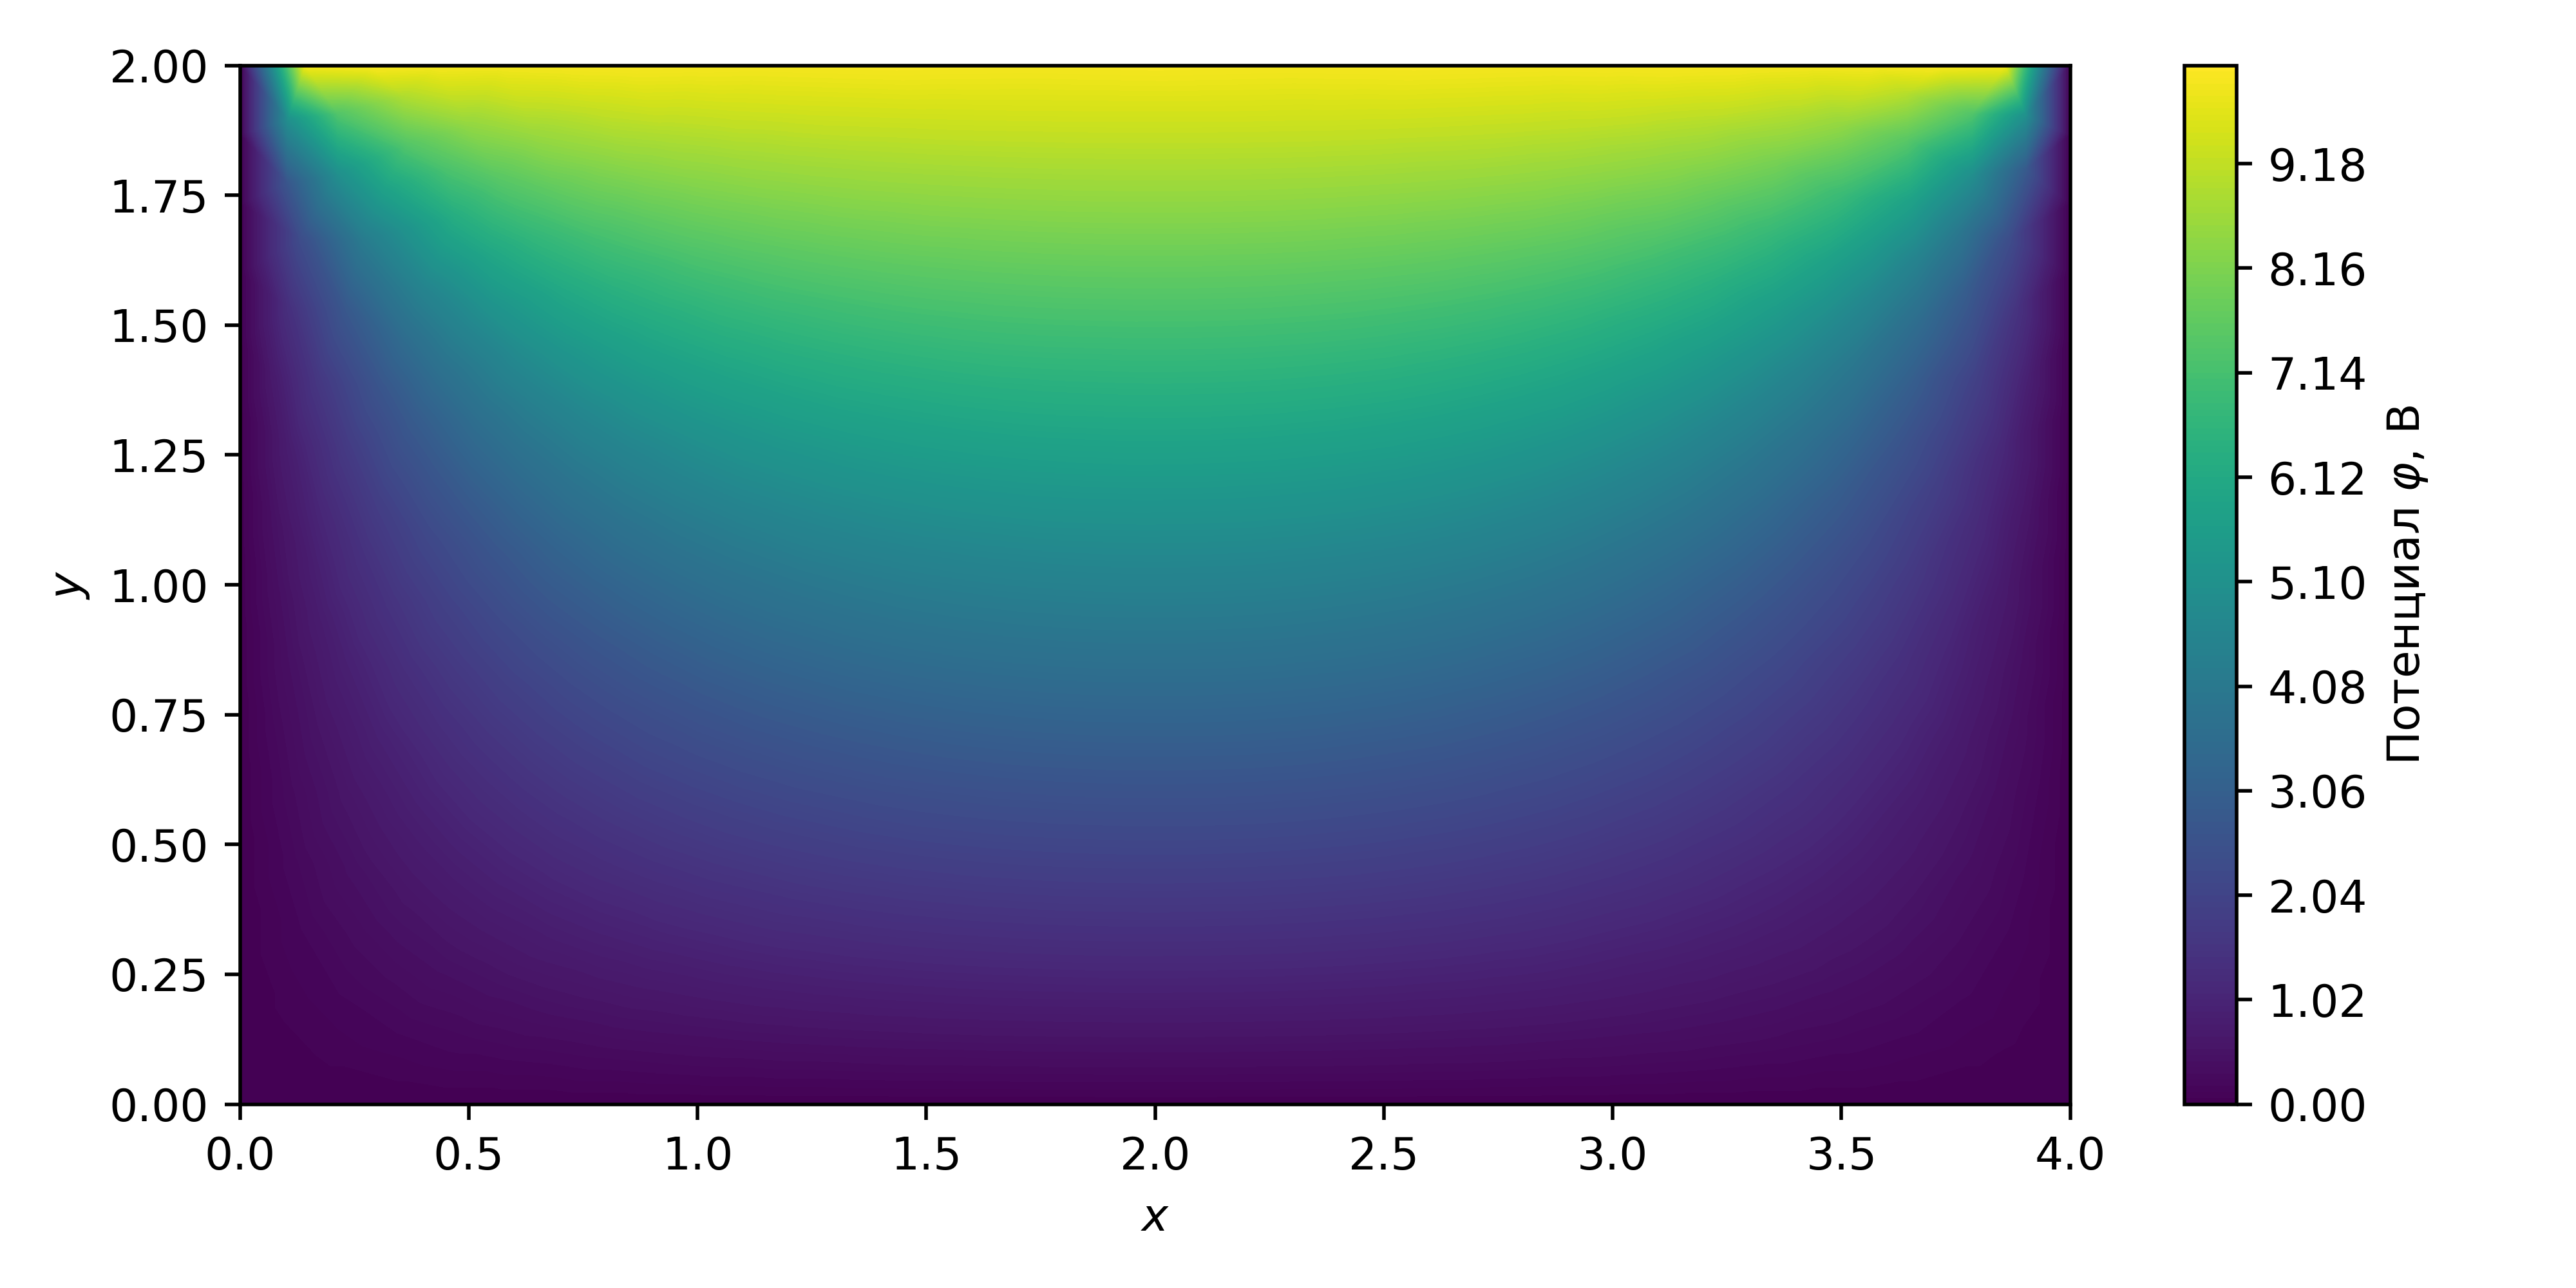
\includegraphics[width=1\textwidth]{rect_dirichlet_only_exact_sol.png}
						\caption{Точное решение задачи №\,1}
						\label{fig:rect_dom_dir_exact}
					\end{figure*}
				
				
				\newpage
				\subsubsection{Решение}
					Численное решение будем искать на сетках с разными размерами конечного элемента: будет варьироваться параметр $S_{max}$, отвечающий за максимальную площадь конечного элемента. 
					Для построения сеток в данном примере использовалась библиотека CALFEM \cite{calfem}, в которой отношение самой длинной и самой короткой сторон треугольного конечного элемента в среднем стремится к 1. 
							
					Полученные сетки с параметром $S_{max}$ равным $0.05, \ 0.01, \ 0.001$ выглядят следующим образом: 
					
					%\newpage
										
					\begin{figure}[h]  
						\centering     
						\vspace{5.0mm} 
						\begin{center} 
							{ 
								\begin{minipage}{0.45\textwidth} 
									\centering 
									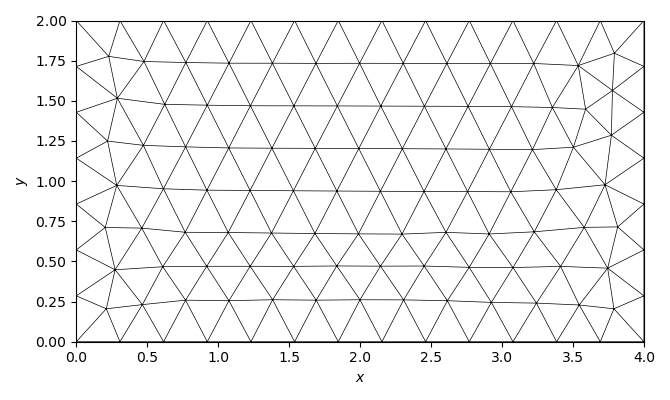
\includegraphics[width=1\columnwidth]{rect_dirichlet_only_005_calfem_net.png}\\ 
									\textit{a} 
								\end{minipage}                                 
							} 
							{ 
								\begin{minipage}{0.45\textwidth} 
									\centering 
									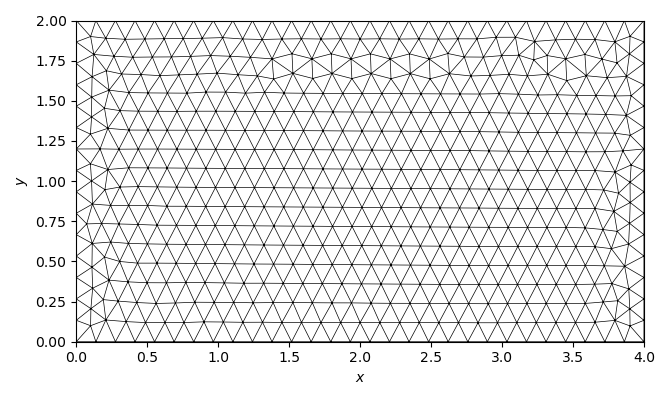
\includegraphics[width=1\columnwidth]{rect_dirichlet_only_001_calfem_net.png}\\ 
									\textit{b} 
								\end{minipage}                                 
							} 
							{ 
								\begin{minipage}{0.7\textwidth} 
									\centering 
									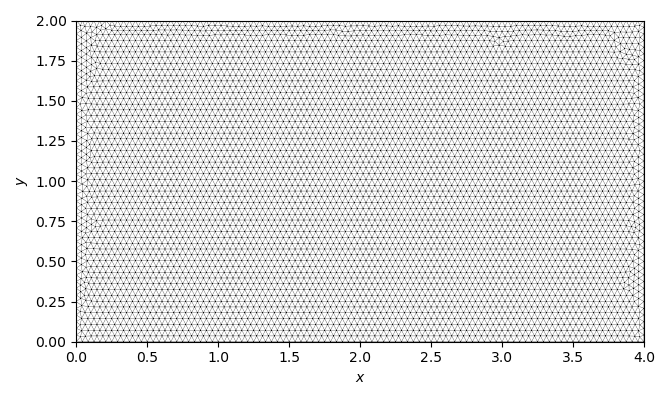
\includegraphics[width=1\columnwidth]{rect_dirichlet_only_0001_calfem_net.png}\\ 
									\textit{c} 
								\end{minipage}                                 
							} 						
						\end{center} 
						\vspace*{-0.0mm} 
						\caption{Иллюстрации разбиения области $\Omega$ задачи №\,1: 
							\textit{a} --- параметр $S_{max} \rightarrow 0.05$;\\
							\textit{b} --- параметр $S_{max} \rightarrow  0.01$;
							\textit{c} --- параметр $S_{max} \rightarrow 0.001$
						} 
						\label{fig: meshs_for_rect}
					\end{figure}
					
					\looser{-0.02}{Для того, чтобы в дальнейшем качественно сравнить результаты, граничные условия для алгоритма МКЭ будут задаваться с помощью точного решения. Тогда решения поставленной задачи, полученные на сетках рис. }\ref{fig: meshs_for_rect}, выглядят следующим образом:
		
			
			
			
			%\newpage
			
			%Решение задачи №\,1 при разбиение $\Omega$ с параметром $S_{max} \rightarrow 0.05$ выглядит следующим образом: 
			%\vspace*{-5mm}
			\begin{figure*}[!h]
				\centering
				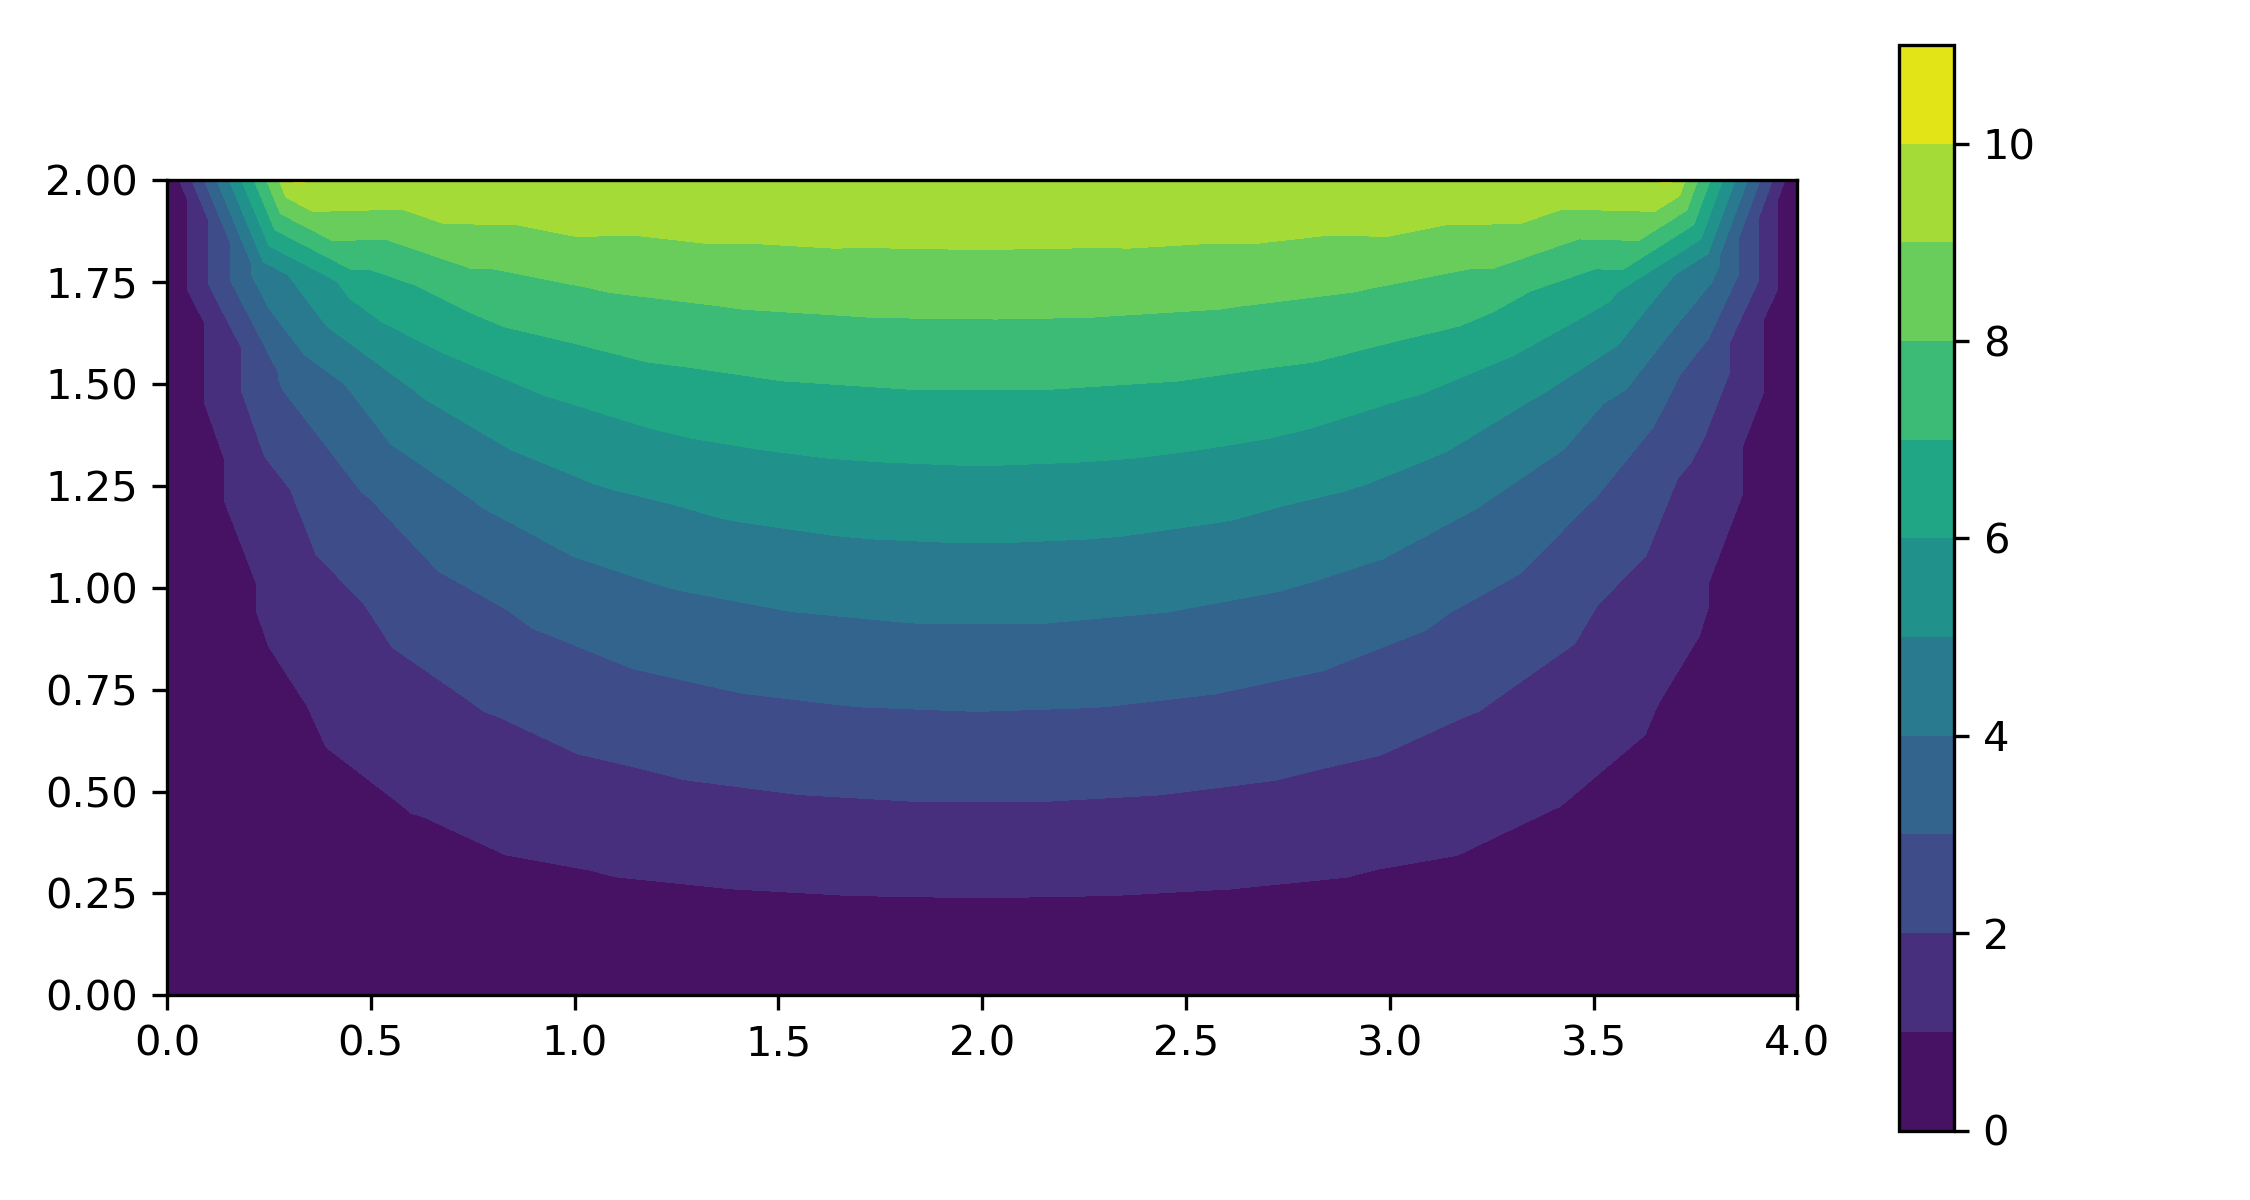
\includegraphics[width=0.75\textwidth]{rect_dirichlet_only_005_calfem.png}
				\caption{Численное решение задачи №\,1 с разбиением области $\Omega$ на элементы с параметром $S_{max} \rightarrow 0.05$}
				\label{fig:dom_rect_005}
			\end{figure*}
			
			% %{	\noindent
			% \begin{table}[!h]
			% 	\centering
			% 	\caption{\label{table_comparison_005} Сравнение значений точного решения и численного решения с разбиением области $\Omega$ с параметром $S_{max} \rightarrow 0.05$  задачи №\,1}
			% 	\vspace*{2mm}
			% 	\begin{tabular}{|c|c|c|c|c|c|}
			% 		\hline
			% 		Узел №
			% 		& Точное решение
			% 		& Приближенное решение 
			% 		& \begin{tabular}[c]{@{}l@{}}Абсолютная \\ погрешность\end{tabular} 
			% 		& \begin{tabular}[c]{@{}l@{}}Относительная \\ погрешность\end{tabular} \\ 				
					
			% 		\hline
			% 		40
			% 		& 1.27392652
			% 		& 1.25634191 
			% 		& 0.01758461
			% 		& 0.01380348 \\ 
					
					
			% 		\hline
			% 		60
			% 		& 3.72330814
			% 		& 3.70649274 
			% 		& 0.0168154
			% 		& 0.00451625 \\ 
					
					
			% 		\hline
			% 		80
			% 		& 1.95722711
			% 		& 1.93729186 
			% 		& 0.01993525
			% 		& 0.01018546 \\ 
					
					
			% 		\hline
			% 		100
			% 		& 2.69063261
			% 		& 2.68065981 
			% 		& 0.0099728
			% 		& 0.00370649 \\ 
					
					
			% 		\hline
			% 		120
			% 		& 1.9138927
			% 		& 1.90537176 
			% 		& 0.00852094
			% 		& 0.00445215 \\ 
					
			% 		\hline
			% 	\end{tabular}				
			% \end{table}		
				
			% \noindent
			% Количество конечных элементов: 216.\\
			% Средняя площадь элемента:  0.04. \\
			% Максимальная площадь элемента:  0.05. \\
			% Среднее значение абсолютной погрешности: 	0.01087074.\\
			% Среднее значение относительной погрешности: 0.02889112. \\
			% Максимальное значение абсолютной погрешности: 0.66276194. \\			
			% Погрешность в норме $L_2$: 0.05392223. \\
			
			
			%\newpage
			
			%Решение задачи №\,1 при разбиение $\Omega$ с параметром $S_{max} \rightarrow 0.01$ выглядит следующим образом: 
			%\vspace*{-5mm}
			\begin{figure*}[!h]
				\centering
				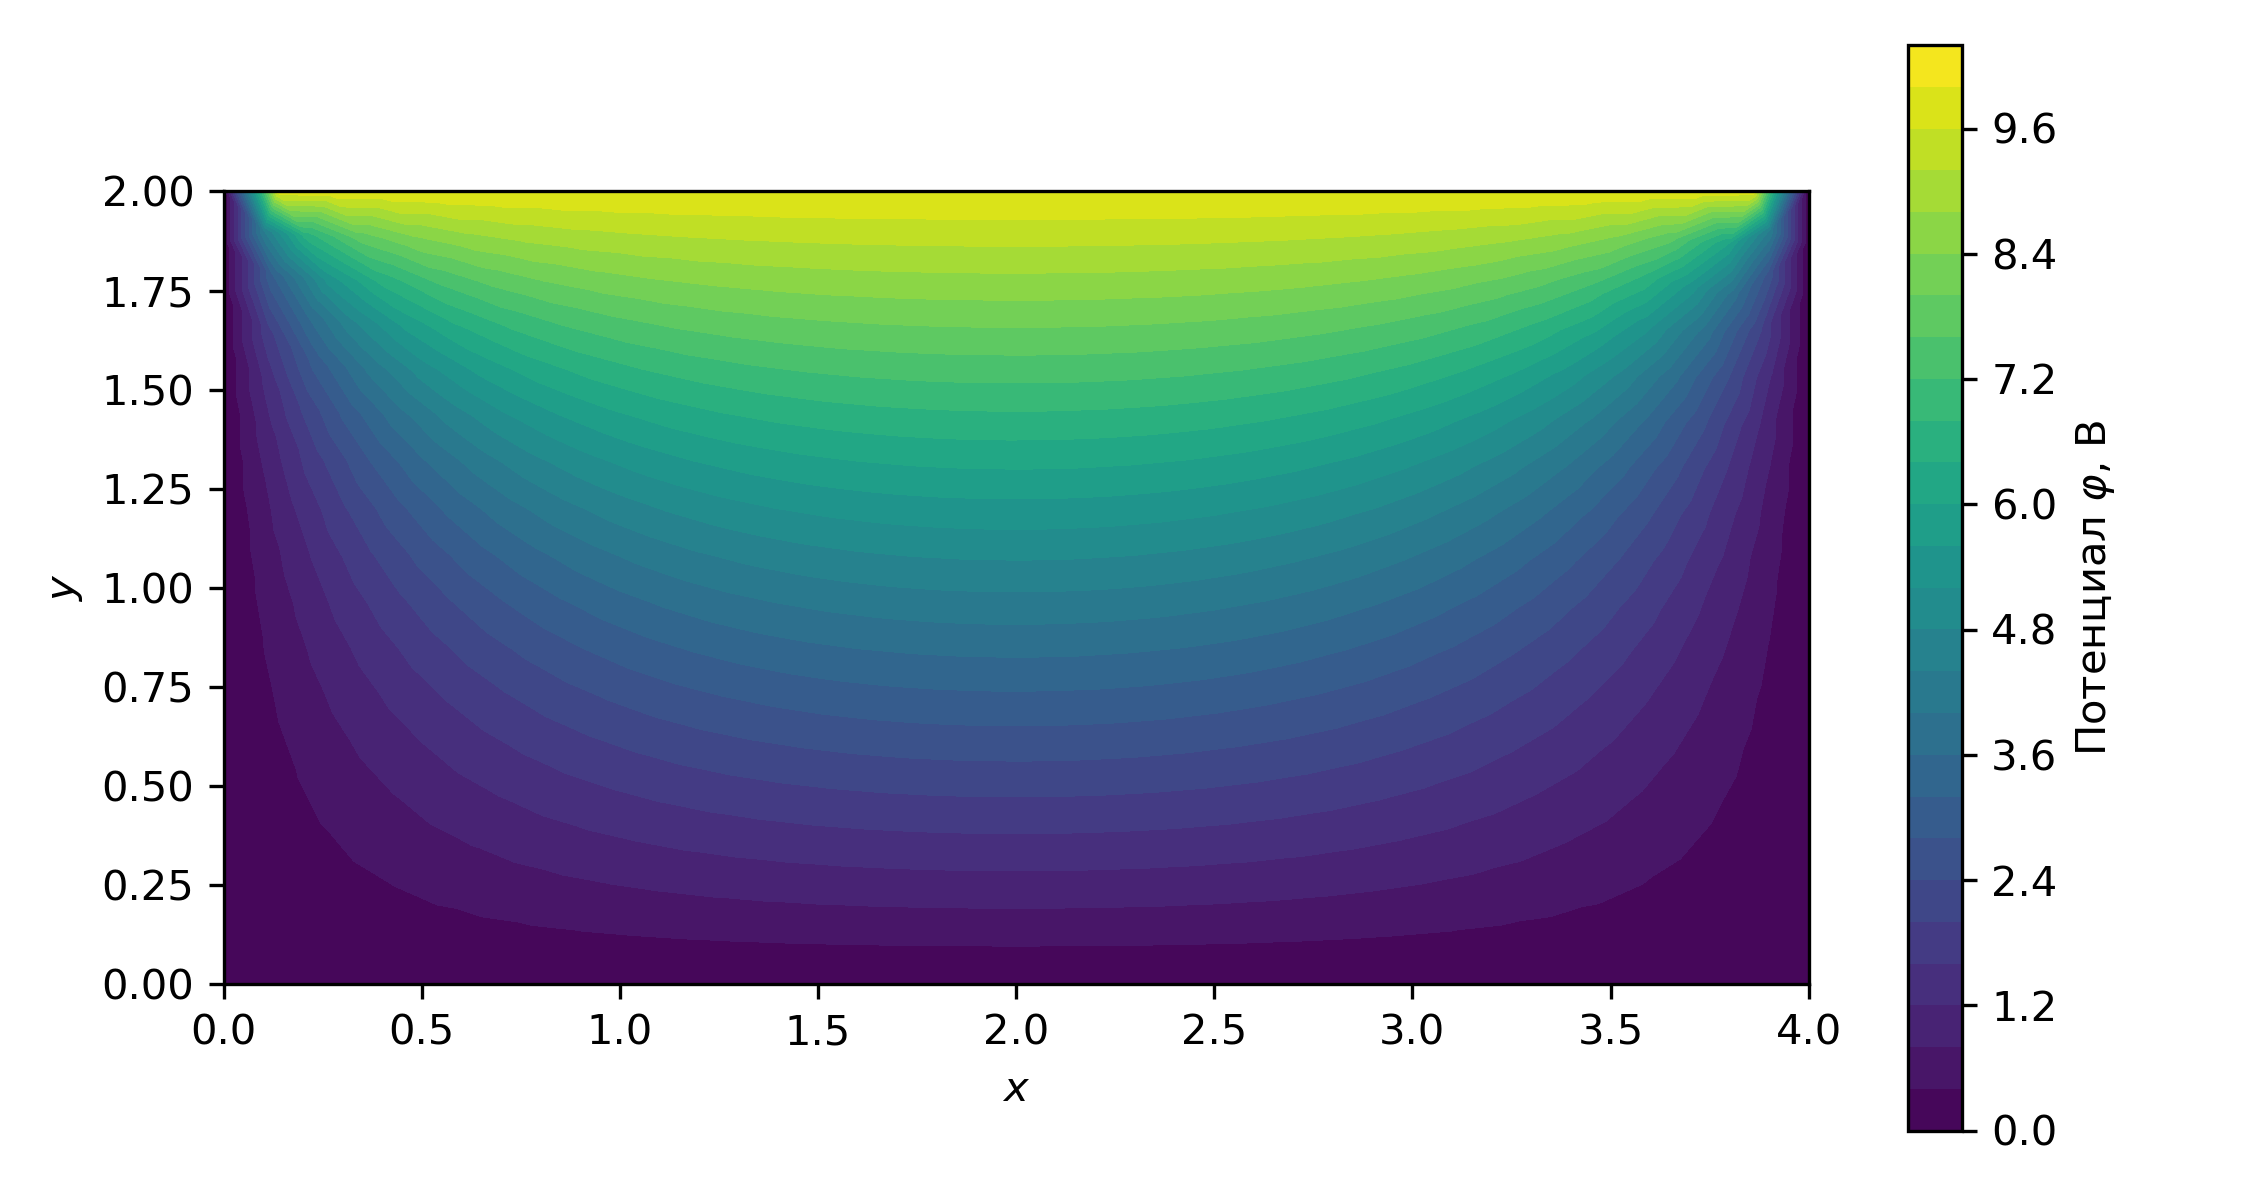
\includegraphics[width=0.75\textwidth]{rect_dirichlet_only_001_calfem.png}
				\caption{Численное решение задачи №\,1 с разбиением области $\Omega$ на элементы с параметром $S_{max} \rightarrow 0.01$}
				\label{fig:dom_rect_001}
			\end{figure*}
			
			
			% \noindent
			% \begin{table}[!h]
			% 	\centering
			% 	\caption{\label{table_comparison_001} Сравнение значений точного решения и численного решения с разбиением области $\Omega$ с параметром $S_{max} \rightarrow 0.01$  задачи №\,1}
			% 	\vspace*{2mm}
			% 	\begin{tabular}{|c|c|c|c|c|c|}
			% 		\hline
			% 		Узел №
			% 		& Точное решение
			% 		& Приближенное решение 
			% 		& \begin{tabular}[c]{@{}l@{}}Абсолютная \\ погрешность\end{tabular} 
			% 		& \begin{tabular}[c]{@{}l@{}}Относительная \\ погрешность\end{tabular} \\ 
									
			% 		\hline
			% 		100
			% 		& 8.79692038
			% 		& 8.7754521 
			% 		& 0.02146828
			% 		& 0.00244043 \\ 
					
					
			% 		\hline
			% 		200
			% 		& 4.20092245
			% 		& 4.18212546 
			% 		& 0.01879699
			% 		& 0.00447449 \\ 
					
					
			% 		\hline
			% 		300
			% 		& 1.26335365
			% 		& 1.26129625 
			% 		& 0.0020574
			% 		& 0.00162853 \\ 
					
					
			% 		\hline
			% 		400
			% 		& 2.55278075
			% 		& 2.5283193 
			% 		& 0.02446145
			% 		& 0.00958228 \\ 
					
					
			% 		\hline
			% 		500
			% 		& 2.88063844
			% 		& 2.68968953 
			% 		& 0.19094891
			% 		& 0.06628701 \\ 
					
			% 		\hline
			% 	\end{tabular}				
			% \end{table}		
			% \vspace*{-5mm}
			
			% \noindent
			% Количество конечных элементов: 1020.\\
			% Средняя площадь элемента:  0.008. \\
			% Максимальная площадь элемента:  0.01. \\
			% Среднее значение относительной погрешности: 0.00395515. \\
			% Среднее значение абсолютной погрешности: 	0.01213012.\\			
			% Максимальное значение абсолютной погрешности: 0.66741336. \\			
			% Погрешность в норме $L_2$: 0.01467814. \\
			
			
			%\newpage
			
			%Решение задачи №\,1 при разбиение $\Omega$ с параметром $S_{max} \rightarrow 0.001$ выглядит следующим образом: 
			%\vspace*{-5mm}
			\begin{figure*}[!h]
				\centering
				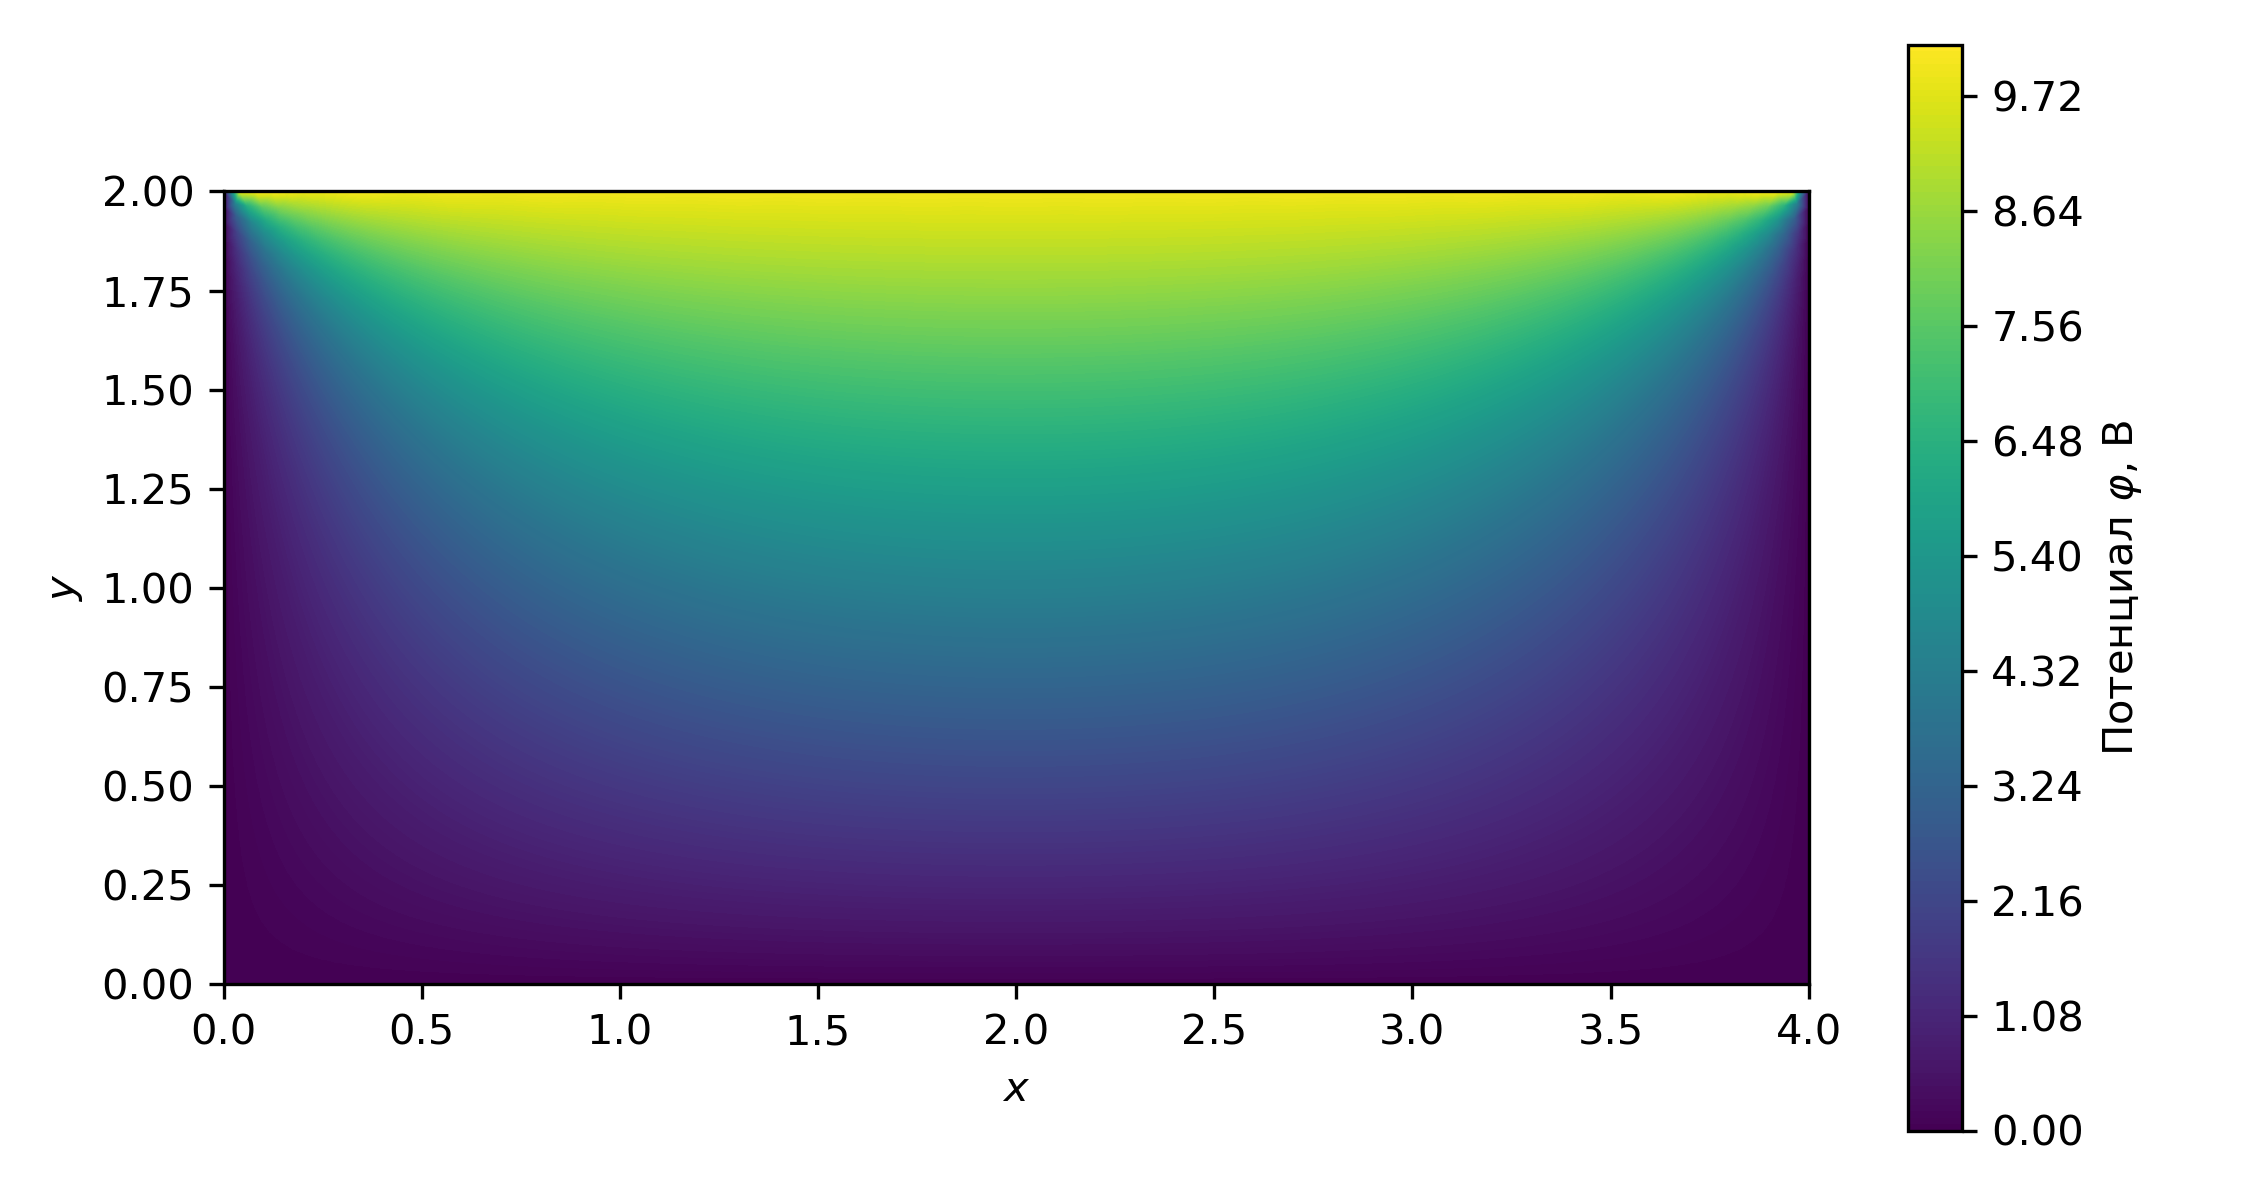
\includegraphics[width=0.75\textwidth]{rect_dirichlet_only_0001_calfem.png}
				\caption{Численное решение задачи №\,1 с разбиением области $\Omega$ на элементы с параметром $S_{max} \rightarrow 0.001$}
				\label{fig:dom_rect_0001}
			\end{figure*}
			
			
			% \noindent
			% \begin{table}[!h]
			% 	\centering
			% 	\caption{\label{table_comparison_0001} Сравнение значений точного решения и численного решения с разбиением области $\Omega$ с параметром $S_{max} \rightarrow 0.001$  задачи №\,1}
			% 	\vspace*{2mm}
			% 	\begin{tabular}{|c|c|c|c|c|c|}
			% 		\hline
			% 		Узел №
			% 		& Точное решение
			% 		& Приближенное решение 
			% 		& \begin{tabular}[c]{@{}l@{}}Абсолютная \\ погрешность\end{tabular} 
			% 		& \begin{tabular}[c]{@{}l@{}}Относительная \\ погрешность\end{tabular} \\ 
					
			% 		\hline
			% 		1000
			% 		& 7.01809786
			% 		& 7.0179319 
			% 		& 0.00016596
			% 		& 2.365e-05 \\ 
					
					
			% 		\hline
			% 		2000
			% 		& 3.09142766
			% 		& 3.09091957 
			% 		& 0.00050809
			% 		& 0.00016436 \\ 
					
					
			% 		\hline
			% 		3000
			% 		& 2.36605127
			% 		& 2.36557367 
			% 		& 0.0004776
			% 		& 0.00020185 \\ 
					
					
			% 		\hline
			% 		4000
			% 		& 6.36926022
			% 		& 6.36913706 
			% 		& 0.00012316
			% 		& 1.934e-05 \\ 
					
					
			% 		\hline
			% 		5000
			% 		& 4.37751466
			% 		& 4.37639743 
			% 		& 0.00111723
			% 		& 0.00025522 \\ 
					
			% 		\hline
			% 	\end{tabular}				
			% \end{table}		
			% \vspace*{-5mm}
			
			% \noindent
			% Количество конечных элементов: 10778.\\
			% Средняя площадь элемента:  0.0007. \\
			% Максимальная площадь элемента:  0.001. \\
			% Среднее значение относительной погрешности: 0.00030776. \\
			% Среднее значение абсолютной погрешности: 	0.00107663.\\			
			% Максимальное значение абсолютной погрешности: 0.62899979. \\			
			% Погрешность в норме $L_2$: 0.00096066. \\
		 	
	 	\newpage
	 	
	 	\subsubsection{Оценка погрешности аппроксимации решения}
	 	Для оценки погрешности полученного решения $u_{approx}$ относительно точного решения $u_{exact}$ возьмем среднее значении абсолютной погрешности по всем узлам (\ref{abs_err}) и квадрат погрешности решения в норме $L_2$ (\ref{l2_err}):
	 	\begin{equation}
	 		\mathrm{avg}(\mathrm{AbsErr}) = \dfrac{1}{N} \sum_{i = 1}^{N} \left| u_{exact, i} - u_{approx, i} \right|,
	 		\label{abs_err}
	 	\end{equation}
	 	\looser{0.02}{где $N$ --- количество узлов, $u_{exact, i},\ u_{approx, i}$ --- точное и приближенное решения в $i$-ом узле;}
	 	\begin{equation}
	 		\mathrm{Err}_{L_2}^2 = \| u_{exact} - u_{approx} \|_{L_2}^{2} = \int_S (u_{exact} - u_{approx})^2 dS,
	 		\label{l2_err}
	 	\end{equation}
	 	где $S$ --- площадь области $\Omega$. Численный аналог формулы (\refeq{l2_err}) получается следующим образом:
	 	\begin{gather*}
	 		\int_S (u_{exact} - u_{approx})^2 dS = \sum_{i = 1}^{N_{el}} \int_{S_i} (u_{exact} - u_{approx})^2 dS, \\
	 		\int_{S_i} (u_{exact} - u_{approx})^2 dS \approx \dfrac{S_i}{N_v} \sum_{j = 1}^{N_v}  (u_{exact,\,ij} - u_{approx,\,ij})^2, \\
	 		u_{approx,\,ij} = \sum_{k = 1}^{N_v} u_{approx,\,ij} \, \phi_{ik},		
	 	\end{gather*} 
	 	\looser{0.0115}{где 
	 		где $N_{el}$ --- количество конечных элементов,
	 		$S_i$ --- площадь $i$-ого конечного элемента, $N_v$ --- количество узлов конечного элемента, $u_{exact,\,ij},\ u_{approx,\,ij}$ --- точное и приближенное значения решения в $j$-ом узле $i$-ого элемента, $\phi_{ik}$ --- базисная функция в $k$-ом узле $i$-ого конечного элемента.} 
	 	
	 	Так как в качестве конечного элемента выбран треугольный элемент, а базисные функции такие, что имеют значение 1 в своем узле и 0 во всех остальных, то формула для вычисления погрешности решения в норме $L_2$ примет вид
	 	\begin{equation}
	 		\mathrm{Err}_{L_2}^2 \approx \sum_{i = 1}^{N_{el}} S_i
	 		\sum_{j = 1}^{3}  \dfrac{\phantom{|}(u_{exact,\,ij} - u_{approx,\,ij})^2}{3}.
	 		\label{l2_err_approx}
	 	\end{equation}
	 	%Для более точного исследования погрешности метода, для вычисления значений на границах области будет использоваться точное решение (\refeq{exact_solution}).
			
	
	
	
		\newpage
				
		\subsubsection{Погрешность аппроксимации на сетках}
			
			Для анализа качества аппроксимации дополнительно построим решения на сетках с параметром $S_{max}$ равным 0.005, 0.0005. 
			
			\vspace*{-1mm}
			\begin{table}[!h]
				\centering
				\caption{\label{table_comparison} Оценка погрешности аппроксимации решения в зависимости от максимальной площади конечного элемента для задачи №\,1}
				\vspace*{2mm}
				%\hspace*{-8mm}
				\begin{NiceTabular}{|c|c|c|c|c|}[colortbl-like]
					
					\hline
					\multicolumn{1}{|c|}{\begin{tabular}[c]{@{}c@{}c@{}}
					Количество\\ 
					конечных \\ 
					элементов\end{tabular}}
					& \begin{tabular}[c]{@{}c@{}c@{}}Максимальная \\ площадь конечного\\  элемента, $S_{max}$ \end{tabular}
					& \begin{tabular}[c]{@{}c@{}c@{}}Средняя длина\\ ребра конечного\\  элемента, $h$ \end{tabular}
					% & \multicolumn{1}{c|}{\begin{tabular}[c]{@{}c@{}c@{}}Среднее значение\\ абсолютной\\ погрешности\end{tabular}}
					& $\mathrm{avg}(\mathrm{AbsErr})$
					& $\mathrm{Err}_{L_2}^2$  \\
					% \begin{tabular}[c]{@{}c@{}}Погрешность \\ решения\\ в норме $L_2$\end{tabular} \\ 
					
					\hline
					216
					& 0.05
					& 0.3
					& 0.0289 
					& 0.0539 \\ 
					
					
					\hline
					1020
					& 0.01
					& 0.135
					& 0.0121
					& 0.0147 \\ 
					
						
					\hline
					1874
					& 0.005
					& 0.1
					& 0.0044
					& 0.0042 \\
					
					\hline
					10778
					& 0.001
					& 0.041
					& 0.00107
					& 0.00096 \\ 
					
					\hline
					22124
					& 0.0005
					& 0.029
					& 0.00053 
					& 0.00046 \\ 
					
					\hline
				\end{NiceTabular}
				\label{table: 4}				
			\end{table}		
			\vspace*{2mm}
			
			Из таблицы \ref{table: 4} видно, что $\mathrm{avg}(\mathrm{AbsErr})$ и
			$\mathrm{Err}_{L_2}^2$ являются величинами порядка $O(h^2)$ или же $O(S_{max})$ и меняются линейно в зависимости от площади конечного элемента.
		 
			Исследуем зависимость погрешности решения от отношение самой длинной и самой короткой сторон треугольного конечного элемента. Для этого построим сетки с помощью Wolfram Mathematica, c параметром $S_{max}$ равным 0.05, 0.01, 0.001.
			
			
			\begin{figure}[h]  
				\centering     
				\vspace{-2.0mm} 
				\begin{center} 
					{ 
						\begin{minipage}{0.47\textwidth} 
							\centering 
							\hspace*{-17.7mm}
							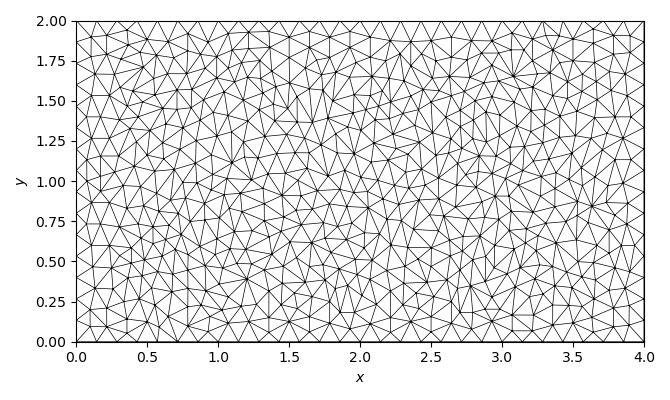
\includegraphics[width=1.2\columnwidth]{rect_dirichlet_only_001_net.png}\\ 
							\hspace*{-11mm}
							\textit{a} 
						\end{minipage}                                 
					} 
					{ 
						\begin{minipage}{0.47\textwidth} 
							\centering 
							\hspace*{-7.2mm}
							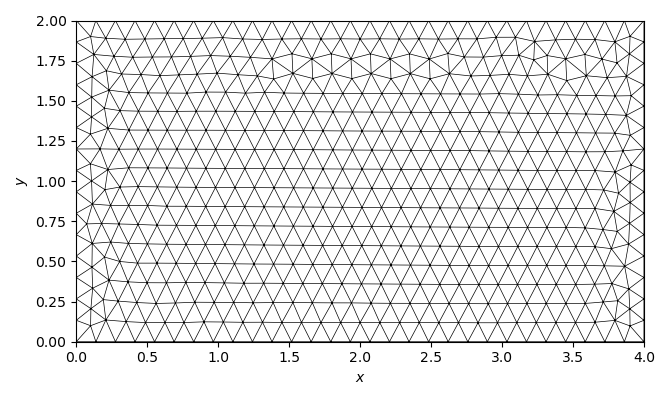
\includegraphics[width=1.2\columnwidth]{rect_dirichlet_only_001_calfem_net.png}\\
							\hspace*{7.2mm} 
							\textit{b} 
						\end{minipage}                                 
					} 				
				\end{center} 
				\vspace*{-0.0mm} 
				\caption{Иллюстрации разбиения области $\Omega$ задачи №\,1 с параметром $S_{max} \rightarrow 0.01$: \\
					\textit{a} --- сетка Wolfram Mathematica;
					\textit{b} --- сетка CALFEM;
				} 
				\label{fig: comp_mesh_calfem_wolfram}
			\end{figure}
			
		%	\begin{figure*}[!h]
		%		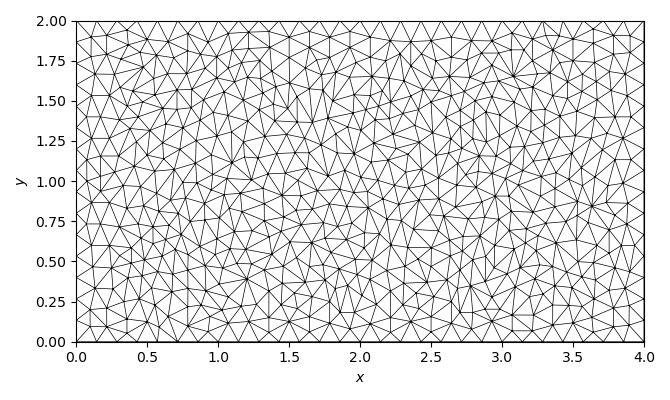
\includegraphics[width=0.7\textwidth]{rect_dirichlet_only_001_net.png}
		%		\caption{Пример сетки построенной в Wolfram Mathematica параметром $S_{max} \rightarrow 0.01$}
		%		\label{fig:dom_rect_005_wolfram}
		%	\end{figure*}
			
			На этапе построения сетки видно, что, в отличие от CALFEM, где в среднем отношение большего и меньшего ребер конечного элемента 
			$\dfrac{h_{max}}{h_{min}} \approx 1.1$, сетка в Wolfram Mathematica выходит менее структурированной, для нее отношение большего и меньшего ребер в среднем равно $\dfrac{h_{max}}{h_{min}} \approx 1.4$. 
			
			
			
			
			\begin{table}[!h]
				\centering
				%\hspace*{-2mm}
				\caption{Сравнение решений задачи №\,1 в зависимости от отношения большего и меньшего ребер конечного элемента}
				\vspace*{2mm}
				\begin{NiceTabular}{|c|c|c|c|c|}[colortbl-like]
					
					\hline
					\rowcolor[HTML]{ededed}\xrowht{20pt}   
					\begin{tabular}[c]{@{}c@{}}Средняя длина\\ ребра конечного\\  элемента, $h$\end{tabular} 
					& $\mathrm{avg} \left( \dfrac{h_{max}}{h_{min}} \right) $
					& $\max \left( \dfrac{h_{max}}{h_{min}} \right) $
					% & \begin{tabular}[c]{@{}c@{}}Среднее значение\\ абсолютной\\ погрешности\end{tabular} 
					& $\mathrm{avg}(\mathrm{AbsErr})$
					& $\mathrm{Err}_{L_2}^2$  \\
					% & \begin{tabular}[c]{@{}c@{}}Погрешность \\ решения\\ в норме $L_2$\end{tabular} \\ 
					\hline\hline
					
					
					0.3                                                                                
					&  1.1                                                                         
					&  1.5                                                                                        
					& 0.03                                                                                
					& 0.05   \\
					\hline
					
					0.3                                                                                
					&  1.4                                                                         
					&  2                                                                                          
					& 0.02                                                                                
					& 0.034  \\
					\hline
					
					
					\rowcolor[HTML]{ededed}\xrowht{5pt}   
					0.135                                                                              
					&  1.1                                                                         
					&  1.4                                                                                        
					& 0.01                                                                                
					& 0.015  \\
					\hline
					
					0.127                                                                   
					\rowcolor[HTML]{ededed}\xrowht{5pt}              
					&  1.4                                                                         
					&  2.3                                                                                        
					& 0.008                                                                               
					& 0.013  \\
					\hline
					
					
					0.04             
					&  1.1                                                                         
					&  1.4                                                                                        
					& 0.001                                                                               
					& 0.001  \\
					\hline
					
					0.04                                                                               
					&  1.4                                                                         
					&  2.3                                                                                        
					& 0.003                                                                               
					& 0.007  \\
					\hline
					
					\rowcolor[HTML]{ededed}\xrowht{5pt}   
					0.038          
					&  1
					&  1.5
					& 0.0007 
					& 0.0004 \\
					\hline
					
					\rowcolor[HTML]{ededed}\xrowht{5pt}   
					0.036           
					&  1.4                                    
					&  2.3
					& 0.0052 
					& 0.0047    \\ 
					\hline
					
				\end{NiceTabular}
				\label{table:vert_comp}
			\end{table}
			\vspace*{5mm}
			Из таблицы видно, что при уменьшении ребра $h$, отношение длин сторон конечного элемента $\mathrm{avg} \left( \dfrac{h_{max}}{h_{min}} \right)$ начинает играть существенную роль.			
			Также отдельно рассмотрим узлы сетки, в которых абсолютная погрешность отличается от своего среднего значения больше чем на $20\%$. 
			\vspace*{5mm}
			\begin{figure}[!h]  
				\centering     
				\vspace{5.0mm} 
				\begin{center} 
					{ 
						\begin{minipage}{0.45\textwidth} 
							\centering 
							\hspace*{-32.7mm}
							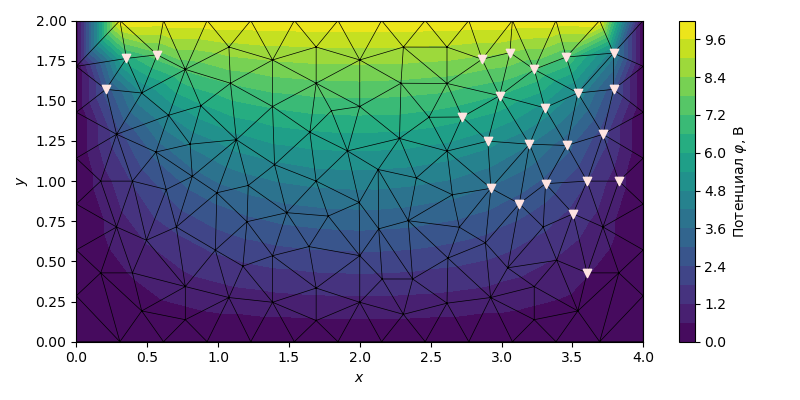
\includegraphics[width=1.4\columnwidth]{rect_dirichlet_only_005_err_nodes.png}\\ 
							\hspace*{-42.7mm}
							\textit{a} 
						\end{minipage}                                 
					} 
					{ 
						\begin{minipage}{0.45\textwidth} 
							\centering 
							\hspace*{-8.2mm}
							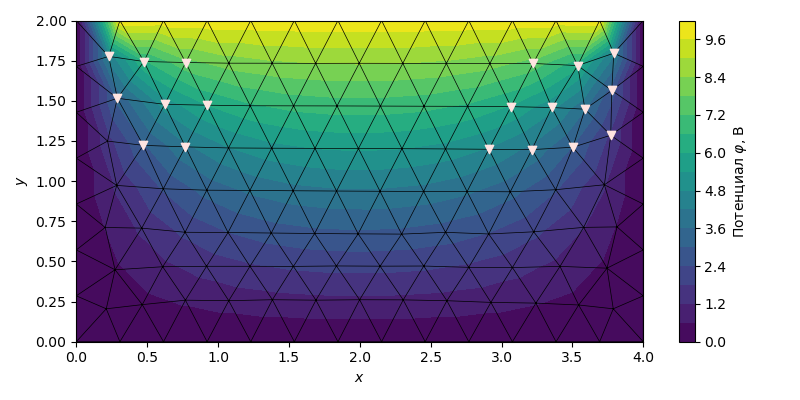
\includegraphics[width=1.4\columnwidth]{rect_dirichlet_only_005_calfem_err_nodes.png}\\ 
							\hspace*{2.2mm}
							\textit{b} 
						\end{minipage}                                 
					} 
									
				\end{center} 
				\vspace*{-0.0mm} 
				\caption{Иллюстрация точек с наибольшим отклонением численного решения от точного для задачи №\,1 с параметром $S_{max} \rightarrow 0.05$: 
					\textit{a} --- на сетке c $\mathrm{avg} \left( \dfrac{h_{max}}{h_{min}} \right) \approx 1.4 $;\\
					\textit{b} --- на сетке c $\mathrm{avg} \left( \dfrac{h_{max}}{h_{min}} \right) \approx 1.1$
				} 
				\label{fig: max_err_005}
			\end{figure}
			
			\newpage
			
			\begin{figure}[!h]  
				\centering     
				\vspace{5.0mm} 
				\begin{center} 
					{ 
						\begin{minipage}{0.45\textwidth} 
							\centering 
							\hspace*{-32.7mm}
							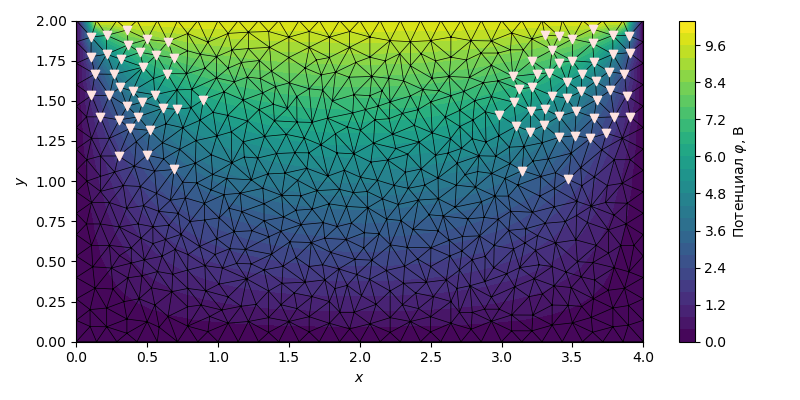
\includegraphics[width=1.4\columnwidth]{rect_dirichlet_only_001_err_nodes.png}\\ 
							\hspace*{-42.7mm}
							\textit{a} 
						\end{minipage}                                 
					} 
					{ 
						\begin{minipage}{0.45\textwidth} 
							\centering 
							\hspace*{-8.2mm}
							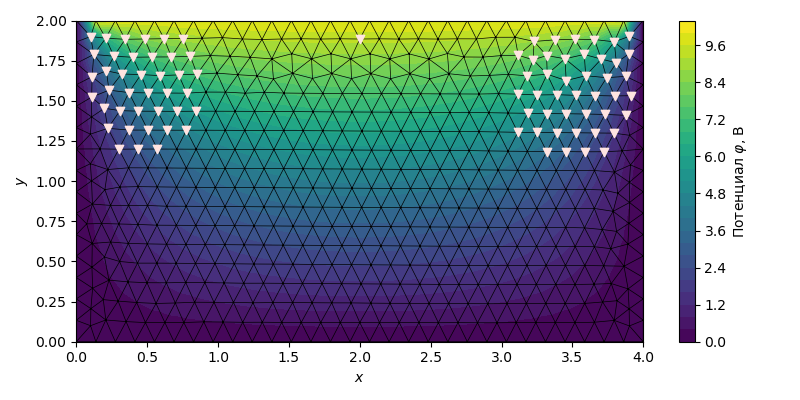
\includegraphics[width=1.4\columnwidth]{rect_dirichlet_only_001_calfem_err_nodes.png}\\
							\hspace*{2.2mm} 
							\textit{b} 
						\end{minipage}                                 
					} 
					
				\end{center} 
				\vspace*{-0.0mm} 
				\caption{Иллюстрация точек с наибольшим отклонением численного решения от точного для задачи №\,1 с параметром $S_{max} \rightarrow 0.01$: 
				\textit{a} --- на сетке c $\mathrm{avg} \left( \dfrac{h_{max}}{h_{min}} \right) \approx 1.4 $;\\
				\textit{b} --- на сетке c $\mathrm{avg} \left( \dfrac{h_{max}}{h_{min}} \right) \approx 1.1$
				} 
				\label{fig: max_err_001}
			\end{figure}
			
			
			\begin{figure}[!h]  
				\centering     
				\vspace{5.0mm} 
				\begin{center} 
					{ 
						\begin{minipage}{0.45\textwidth} 
							\centering 
							\hspace*{-32.7mm}
							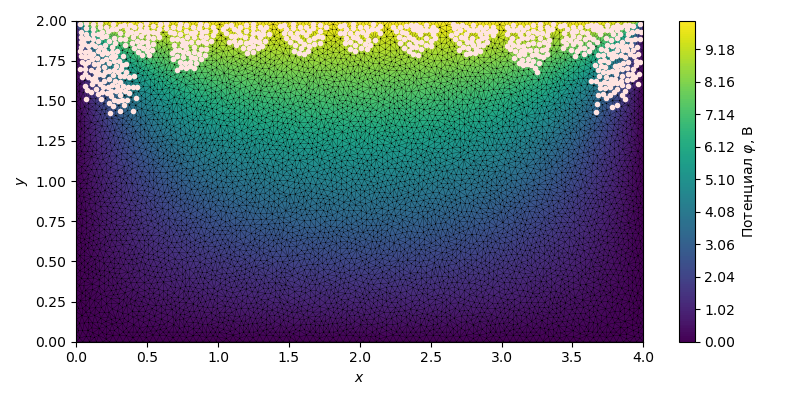
\includegraphics[width=1.4\columnwidth]{rect_dirichlet_only_0001_err_nodes.png}\\ 
							\hspace*{-42.7mm}
							\textit{a} 
						\end{minipage}                                 
					} 
					{ 
						\begin{minipage}{0.45\textwidth} 
							\centering 
							\hspace*{-8.2mm}
							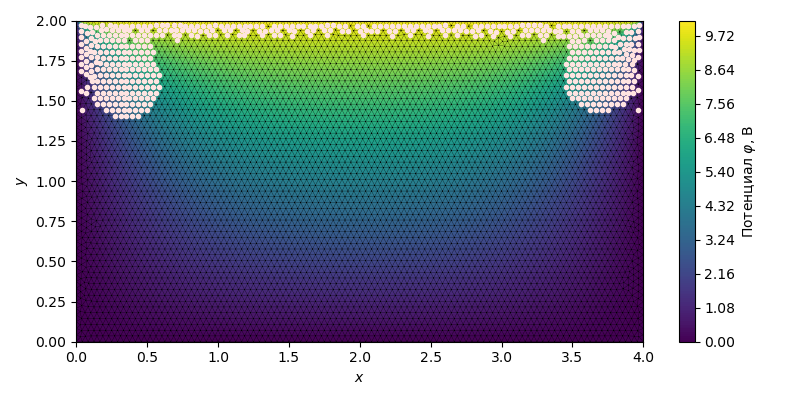
\includegraphics[width=1.4\columnwidth]{rect_dirichlet_only_0001_calfem_err_nodes.png}\\ 
							\hspace*{2.2mm}
							\textit{b} 
						\end{minipage}                                 
					} 
					
				\end{center} 
				\vspace*{-0.0mm} 
				\caption{Иллюстрация точек с наибольшим отклонением численного решения от точного для задачи №\,1 с параметром $S_{max} \rightarrow 0.001$: 
				\textit{a} --- на сетке c $\mathrm{avg} \left( \dfrac{h_{max}}{h_{min}} \right) \approx 1.4 $;\\
				\textit{b} --- на сетке c $\mathrm{avg} \left( \dfrac{h_{max}}{h_{min}} \right) \approx 1.1$
				} 
				\label{fig: max_err_0001}
			\end{figure}
			
			
			
			Как видно из таблицы \ref{table:vert_comp} и рисунков \ref{fig: max_err_005}--\ref{fig: max_err_0001} большая погрешность аппроксимации возникает в приграничных областях, где заданы разные значения на границах. Также видно, что на сетке с отношением  $\mathrm{avg} \left( \dfrac{h_{max}}{h_{min}} \right) \approx 1.4 $ ошибка <<проникает>> глубже внутрь области, чем на сетке с отношением $\mathrm{avg} \left( \dfrac{h_{max}}{h_{min}} \right) \approx 1.1 $. 
			
	
	\newpage
	\subsection{Задача №\,2 (периодические граничные условия)}
		\subsubsection{Условие задачи}
			\looser{0.01}{Найти потенциал в области $\Omega = \left\{ -\infty \leqslant x \leqslant \infty, \  w(x) \leqslant y \leqslant 2 \right\}$}, где $w(x)$ --- периодическая функция с периодом $T = 2$, такая что $w(x) = |x - 1| + 1, \forall x \in \left[ 0, 2 \right]$, на верхней пластине потенциал равен 0 В, на нижней --- 10 В.
		\subsubsection{Решение}
			Рассмотрим задачу при $x \in \left[ 0, 2 \right]$. Запишем систему, которую нужно решить:
			\begin{equation*}
				\begin{cases}
					\Delta \phi (x, y)  = 0, \\
					\phi (x, 2) = 0, \\
					\phi (x, w(x)) = 10, \\
					\phi (0, y) = \phi (2, y).\\
				\end{cases}
			\end{equation*}
			
			Тогда численное решение задачи №\,2, полученное методом конечных элементов при разбиение $\Omega$ с параметром $S_{max} \rightarrow 0.01$ выглядит следующим образом: 

			%% TODO: \usepackage{graphicx} required
			%\begin{figure}[!h]
			%	\centering
			%	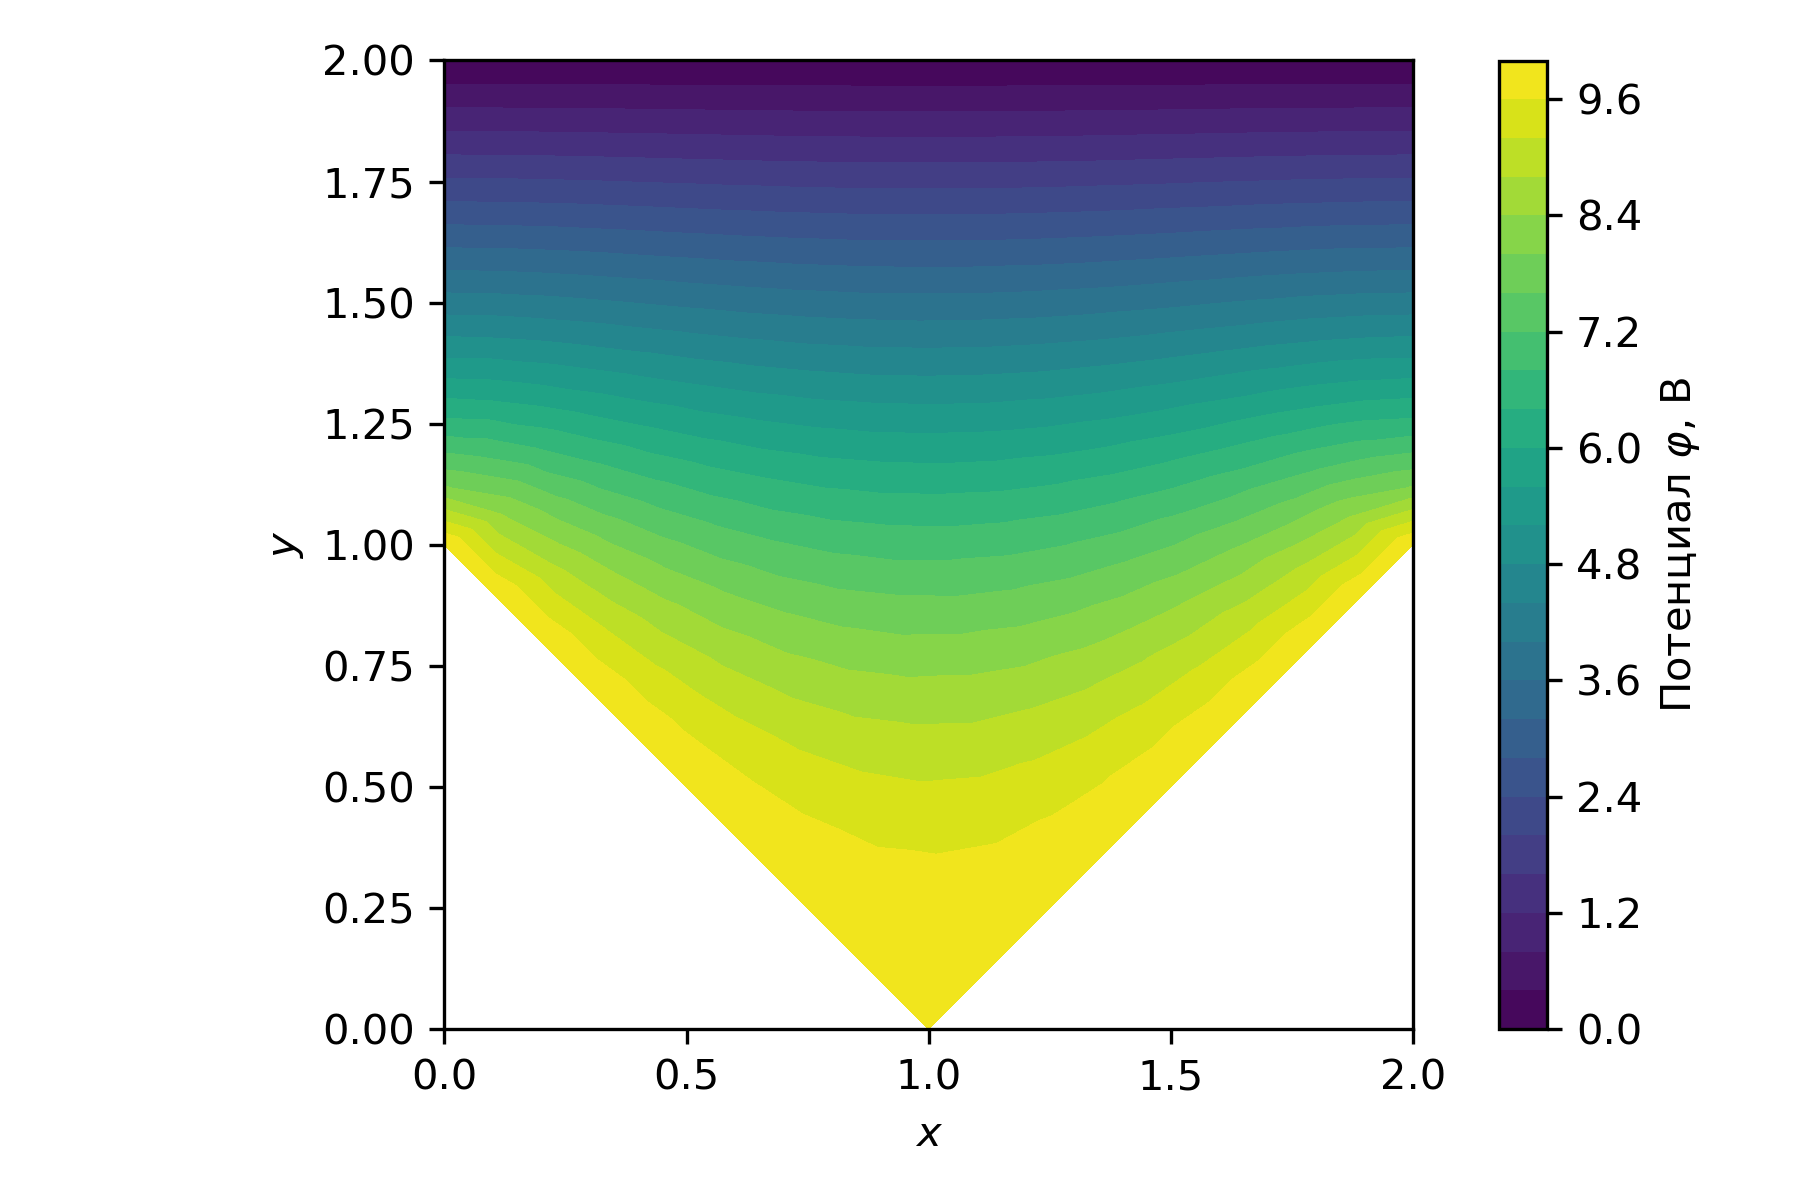
\includegraphics[width=0.7\linewidth]{Test_domain_4_mesh001_calfem.png}
			%	\caption{Численное решение задачи №\,2 с разбиением области $\Omega$ на  элементы с параметром $S_{max} \rightarrow 0.01$}
			%	\label{fig:domain4_mesh001_calfem}
			%\end{figure}
			
			\begin{figure}[h]       
				%\vspace{5.0mm} 
				\begin{center} 
					{ 
						\begin{minipage}{0.47\textwidth} 
							\centering 
							\hspace*{-21.5mm}
							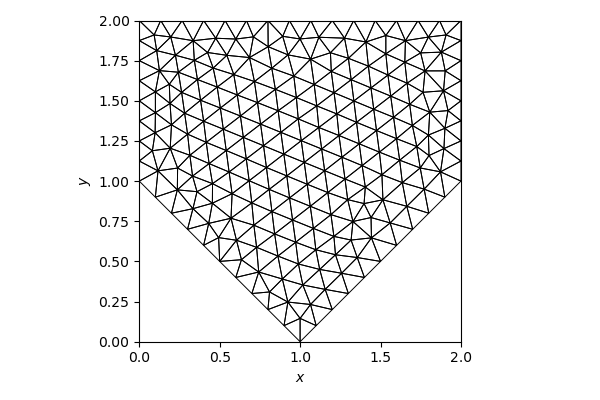
\includegraphics[width=1.4\columnwidth]{Test_domain_4_mesh001_calfem_net_1.png}\\
							\hspace*{-12.5mm}
							\textit{a} 
						\end{minipage}                                 
					} 
					{ 
						\begin{minipage}{0.47\textwidth} 
							\centering 
							\hspace*{-17.5mm}
							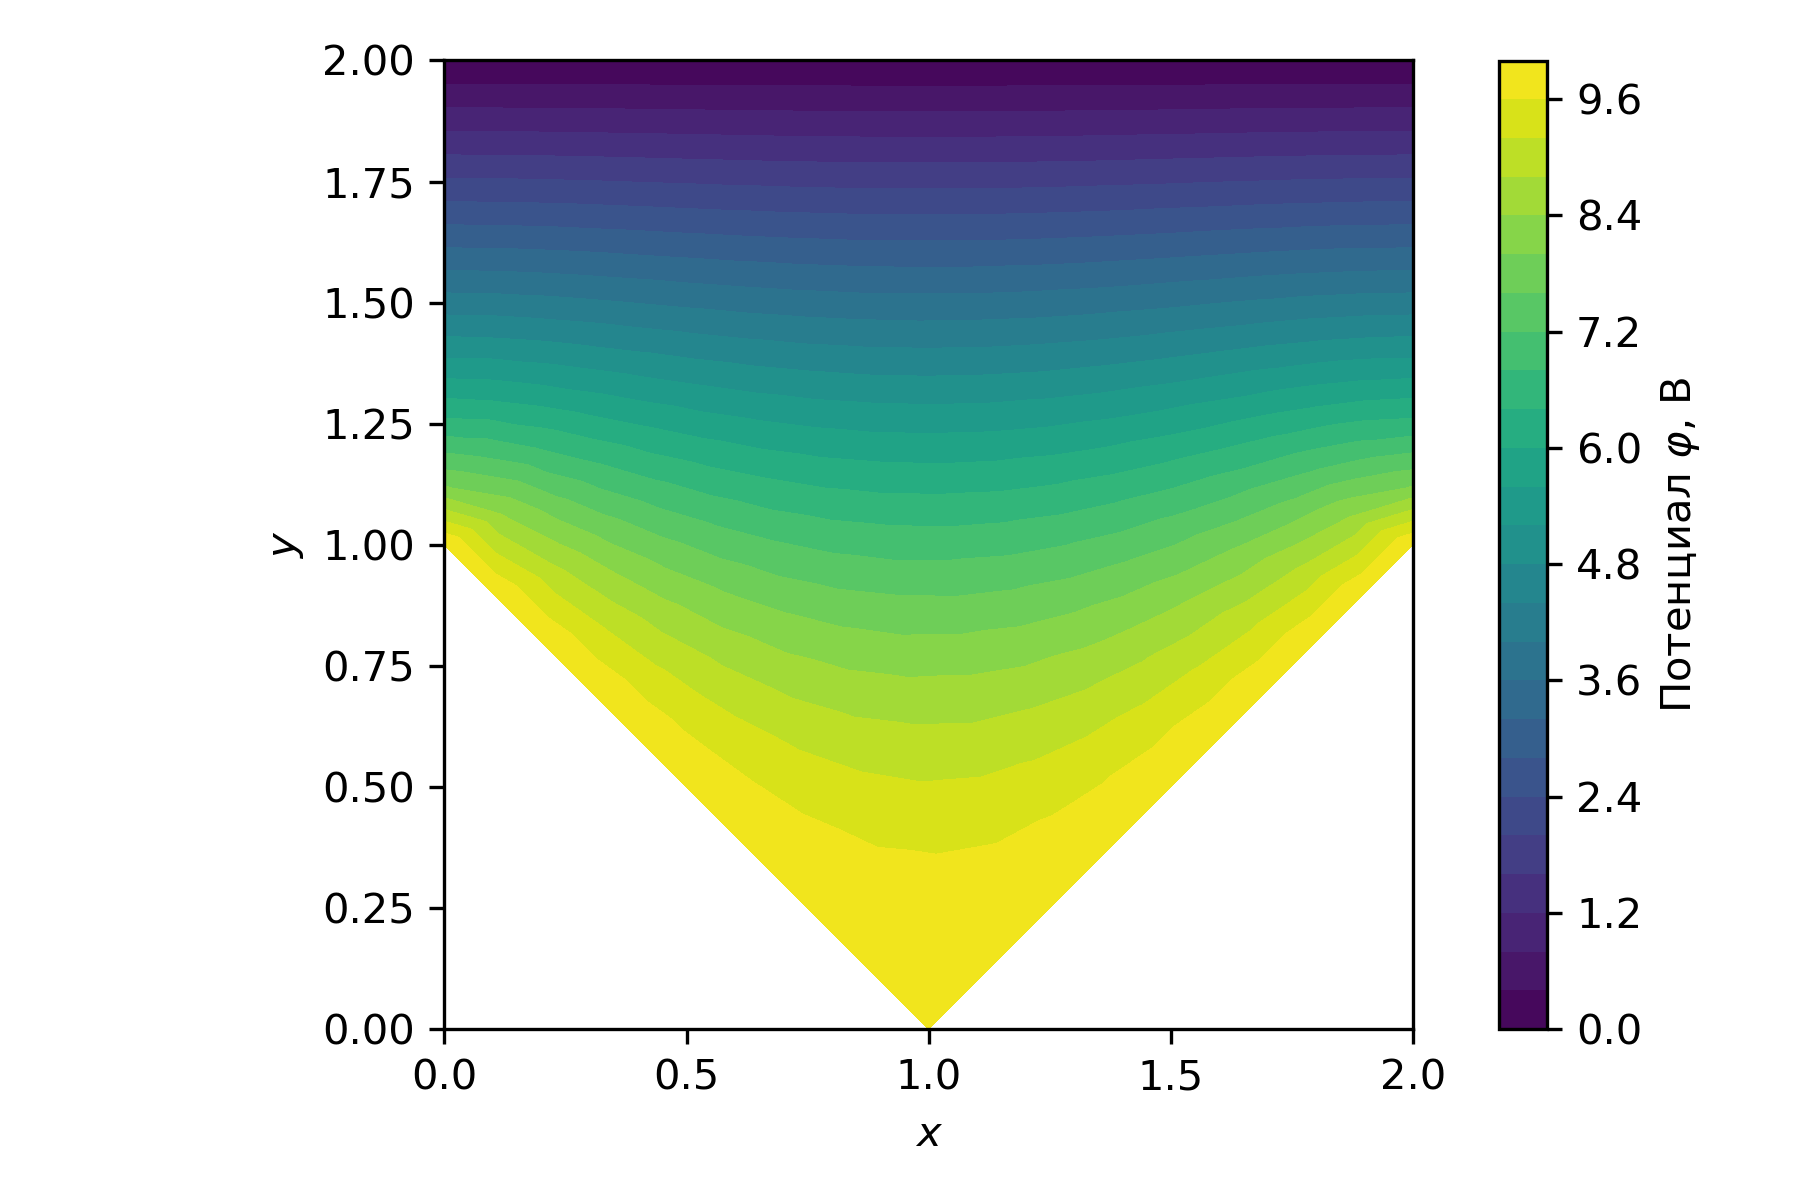
\includegraphics[width=1.4\columnwidth]{Test_domain_4_mesh001_calfem.png}\\
							\hspace*{-1.5mm}
							\textit{b} 
						\end{minipage}                                 
					} 
					
				\end{center} 
				\vspace*{-0.0mm} 
				\caption{Иллюстрации к решению задачи №\,2 на отрезке $\left[ 0, 2 \right]$:\\
					\textit{a} --- иллюстрация разбиения исследуемой области с параметром $S_{max} \rightarrow 0.01$; \\
					\textit{b} --- численное решение задачи №\,2 с разбиением исследуемой области на  элементы с параметром $S_{max} \rightarrow 0.01$ \\
				} 
			\end{figure}
			
			
			
						
			\newpage
			\looser{-0.02}{Аналогично рассмотрим задачу, расширив область поиска решения до трех периодов функции $w(x)$:}
			
			\begin{figure}[h]       
				%\vspace{5.0mm} 
				\begin{center} 
					{ 
						\begin{minipage}{0.9\textwidth} 
							\centering 
							\hspace*{-17mm}
							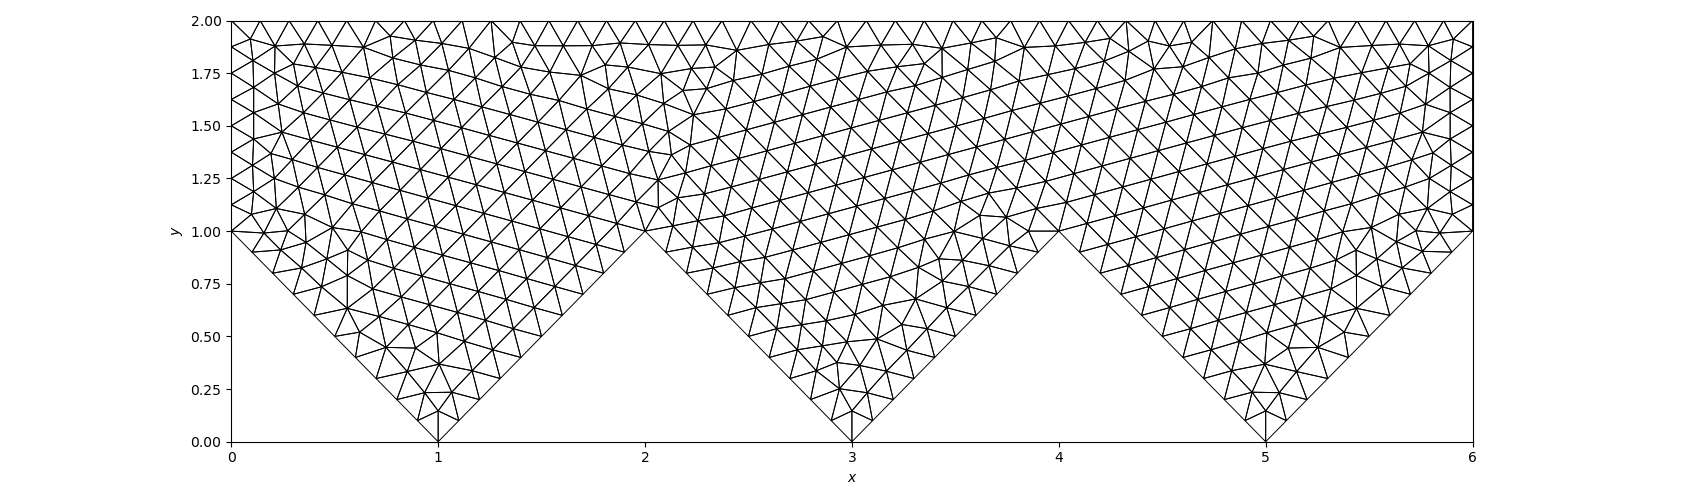
\includegraphics[width=1.2\columnwidth]{Test_domain_4_mesh001_3_in_row_calfem_net_1.png}\\ 
							\textit{a} 
						\end{minipage}                                 
					} 
					{ 
						\begin{minipage}{1\textwidth} 
							\centering 
							\hspace*{-8.5mm}
							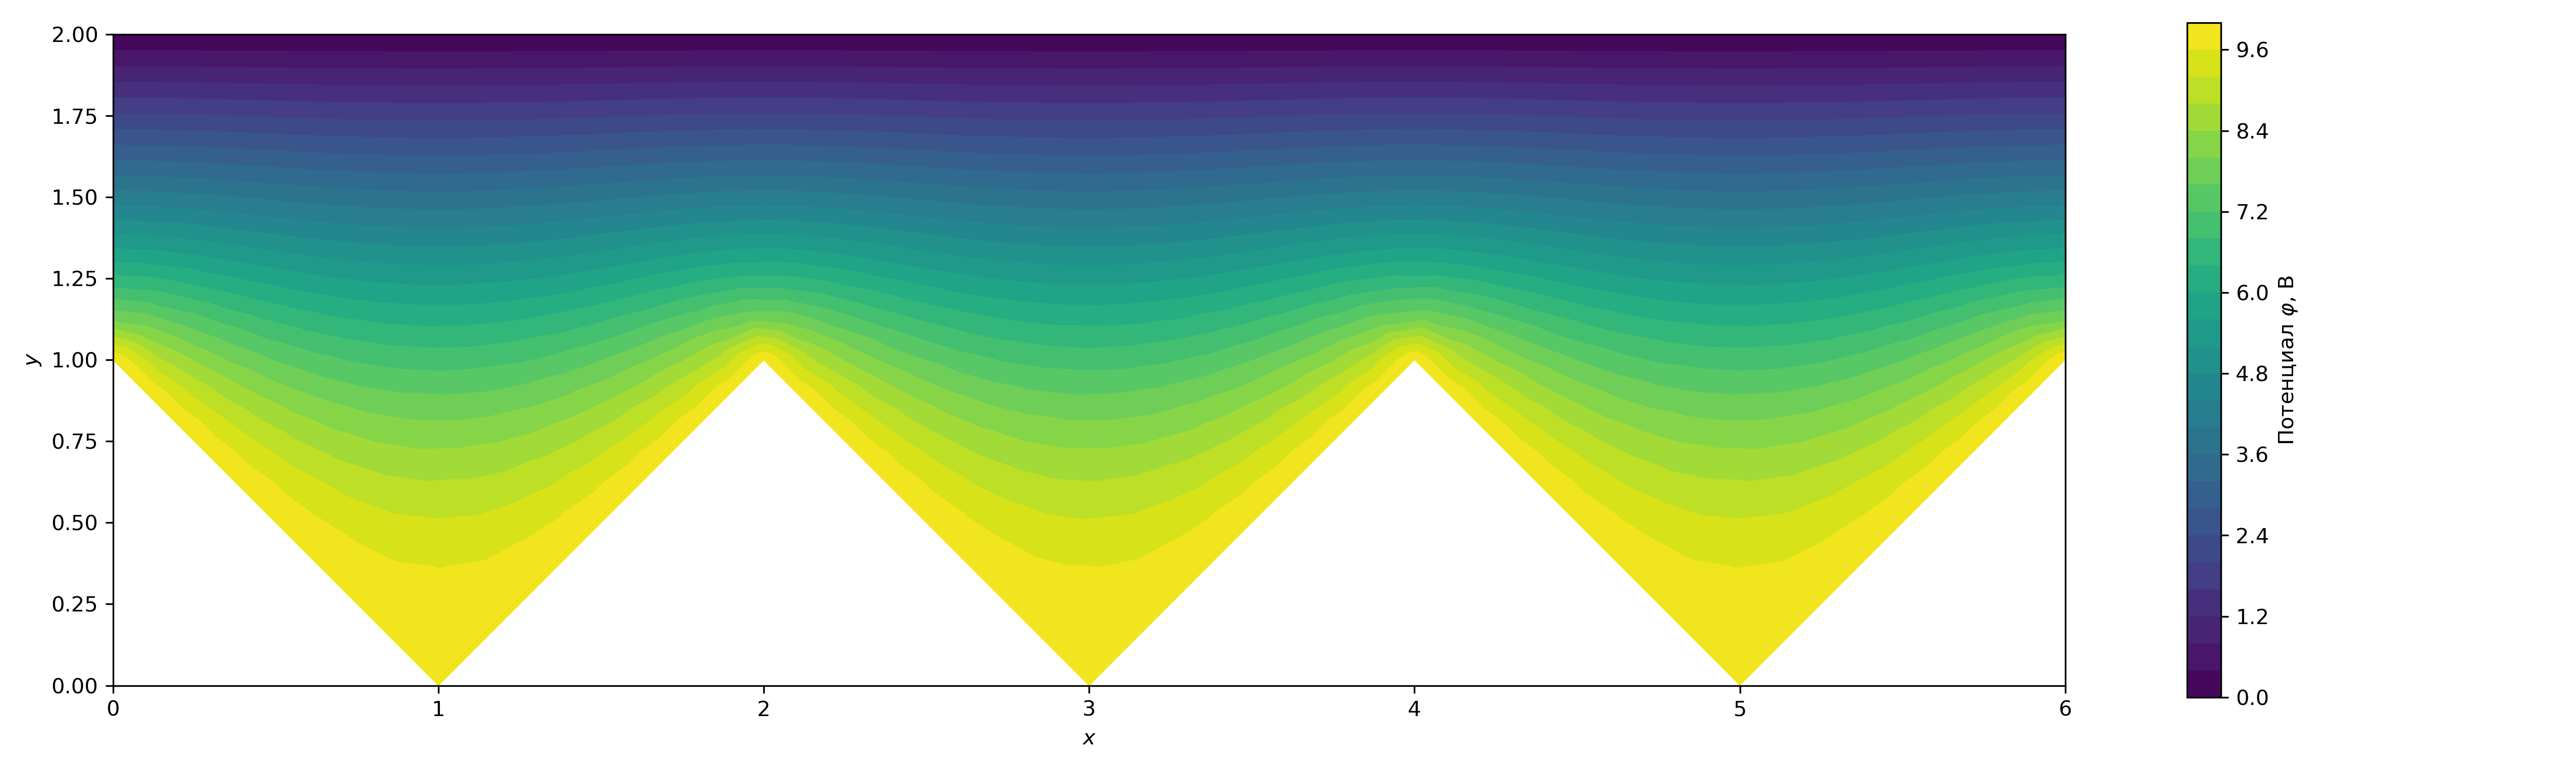
\includegraphics[width=1.2\columnwidth]{Test_domain_4_mesh001_3_in_row_calfem.png}\\ 
							\textit{b} 
						\end{minipage}                                 
					} 
								
				\end{center} 
				\vspace*{-2.0mm} 
				\caption{Иллюстрации к решению задачи №\,2 на отрезке $\left[ 0, 6 \right]$:\\
					\textit{a} --- иллюстрация разбиения исследуемой области с параметром $S_{max} \rightarrow 0.01$; \\
					\textit{b} --- численное решение задачи №\,2 с разбиением исследуемой области на  элементы с параметром $S_{max} \rightarrow 0.01$ \\
				} 
			\end{figure}
			\vspace*{-10mm}
			\subsubsection{Проверка решения на удовлетворение условиям периодичности}
			
				Из графиков видно, что решение гладко меняется внутри области, значения потенциалов в точках
				$(x, w(x))$ и $(x + T, w(x + T))$ выглядят равными. Удостоверимся в этом численно: с помощью формулы интерполирования на треугольной сетке 
				\begin{equation*}
					u(x, y) \approx \sum_{j = 1}^{N} u_{j} \phi_{j}^{xy}, 
				\end{equation*}
				\looser{0.01}{где 
				$N$ --- количество узлов сетки, 
				$u_j$ --- известное значение функции в $j$-ом узле,} 
				$\phi_{j}^{xy}$ --- значение базисной функции в точке $(x, y)$ \cite{Galanin}.
				Вычислим значения в точках, в которых идеологически эти значения должны совпадать. 
				Рассмотрим две группы точек:
				\begin{enumerate}
					\item Точки вида: $(0, y),\ (2, y)$ --- для решения построенного на одном периоде функции $w(x)$,
					$(0, y),\ (2, y),\ (4, y),\ (6, y)$ --- для решения построенного на трех периодах функции $w(x)$:	
				
					\begin{table}[!h]
						\centering
						\caption{ Сравнение\;значений\;численного\;решения\;задачи\;№\,2\;в\;первой\;группе\;точек 
						}
						\vspace*{2mm}
						\begin{NiceTabular}{|c|c|c|}[colortbl-like]
							\hline
							
							\rowcolor[HTML]{ededed}\xrowht{5pt}   
							Область решения
							& Координаты $(x, y)$
							& Значение потенциала $\phi$, В\\
							
							\hline
							\hline
							
							\multirow{2}{*}{1 период $w(x)$}  
							& (0.0, 1.27)                                                      
							& 6.3158	\\ \cline{2-3} 
							
							& (2.0, 1.27)                                                      
							& 6.3158	\\ \hline
							
							
							\rowcolor[HTML]{ededed}\xrowht{5pt}   
							\multirow{4}{*}{3 периода $w(x)$} 
							& (0.0, 1.27)                                                     
							& 6.3093	\\ \cline{2-3} 
							
							\rowcolor[HTML]{ededed}\xrowht{5pt}   
							& (2.0, 1.27)                                                      
							& 6.2896	\\ \cline{2-3} 
							
							\rowcolor[HTML]{ededed}\xrowht{5pt}   
							& (4.0, 1.27)                                                      
							& 6.2946    \\ \cline{2-3} 
							
							\rowcolor[HTML]{ededed}\xrowht{5pt}   
							& (6.0, 1.27)                                                      
							& 6.3093	
							\\ 
							
							\hline
							
							\multirow{2}{*}{1 период $w(x)$}  
							& (0.0, 1.92)                                                      
							& 0.6551	\\ \cline{2-3} 
							& (2.0, 1.92)   
							& 0.6551	\\ 
							
							\hline
							
							
							\rowcolor[HTML]{ededed}\xrowht{5pt}   
							\multirow{4}{*}{3 периода $w(x)$} 
							& (0.0, 1.92)                                                      
							& 0.6547	\\ \cline{2-3} 
							
							\rowcolor[HTML]{ededed}\xrowht{5pt}   
							& (2.0, 1.92)                                                      
							& 0.6549	\\ \cline{2-3}   
							
							\rowcolor[HTML]{ededed}\xrowht{5pt}        
							& (4.0, 1.92)                                                      
							& 0.6555	\\ \cline{2-3}
							 
							\rowcolor[HTML]{ededed}\xrowht{5pt}             
							& (6.0, 1.92)                                                      
							& 0.6547 	\\ \hline
							
							
							
						\end{NiceTabular}
					
						
					\end{table}
					
					\item Точки вида $(1, y)$ --- для решения построенного на одном периоде функции $w(x)$,
					\looser{-0.02}{$(1, y),\ (3, y),\ (5, y)$ --- для решения построенного на трех периодах функции $w(x)$:}
					
					\begin{table}[!h]
						\centering
						\caption{ Сравнение\;значений\;численного\;решения\;задачи\;№\,2\;во\;второй\;группе\;точек 
						}
						\vspace*{2mm}
						\begin{NiceTabular}{|c|c|c|}[colortbl-like]
							\hline
							\rowcolor[HTML]{ededed} \xrowht{15pt}
							Область решения
							& Координаты $(x, y)$
							& Значение потенциала $\phi$, В\\
							
							\hline
							\hline
							
							1 период $w(x)$                 
							& (1.0, 0.75)                                                     
							& 8.3049           \\ \hline
							
							\rowcolor[HTML]{ededed} \xrowht{5pt}
							\multirow{3}{*}{3 периода $w(x)$} 
							& (1.0, 0.75)         
							& 8.305            \\ \cline{2-3} 
							\rowcolor[HTML]{ededed}\xrowht{5pt}   
							& (3.0, 0.75)                                                      
							& 8.3061           \\ \cline{2-3} 
							\rowcolor[HTML]{ededed}\xrowht{5pt}   
							& (5.0, 0.75)                                                      
							& 8.3055           \\ 
							
							
							\hline
							
							1 период $w(x)$                   
							& (1.0, 1.62)                                                      
							& 2.8561           \\ \hline
							
							\rowcolor[HTML]{ededed}\xrowht{5pt}   
							\multirow{3}{*}{3 периода $w(x)$} 
							& (1.0, 1.62)                                                      
							& 2.8556           \\ \cline{2-3} 
							\rowcolor[HTML]{ededed}\xrowht{5pt}   
							& (3.0, 1.62)                                                      
							& 2.858            \\ \cline{2-3} 
							\rowcolor[HTML]{ededed}\xrowht{5pt}   
							& (5.0, 1.62)                                                      
							& 2.8562           \\ \hline					
							
							
							
						\end{NiceTabular}
					\end{table}
				
				\end{enumerate}
				
				\looser{0.02}{Из таблиц видно, что значения отличаются примерно на порядок $O(h^2)$, что показывает выполнение условий периодичности.}
				
			
	\newpage
	\subsection{Задача №\,3 (периодические граничные условия)}
		\subsubsection{Условие задачи}
			\looser{0.01}{Найти потенциал в области $\Omega = \left\{ -\infty \leqslant x \leqslant \infty, \  w(x) \leqslant y \leqslant 2 \right\}$}, где $w(x)$ --- периодическая функция, такая что $w(x) = \dfrac{1}{2} sin \left(\dfrac{\pi x}{2} \right)$, на верхней пластине потенциал равен $12$ В, на нижней --- $-7$ В.
		\subsubsection{Решение}
			Рассмотрим задачу при $x \in \left[ 1, 5 \right]$. Запишем систему, которую нужно решить:
			\begin{equation*}
				\begin{cases}
					\Delta \phi (x, y)  = 0, \\
					\phi (x, 2) = 12, \\
					\phi (x, w(x)) = -7, \\
					\phi (1, y) = \phi (5, y).\\
				\end{cases}
			\end{equation*}
			
			Тогда численное решение задачи №\,3, полученное методом конечных элементов при разбиение $\Omega$ с параметром $S_{max} \rightarrow 0.001$ выглядит следующим образом: 
			\vspace*{5mm}
			\begin{figure}[h]       
				%\vspace{5.0mm} 
					{ 
						\begin{minipage}{0.47\textwidth} 
							\centering 
							\hspace*{-28.5mm}
							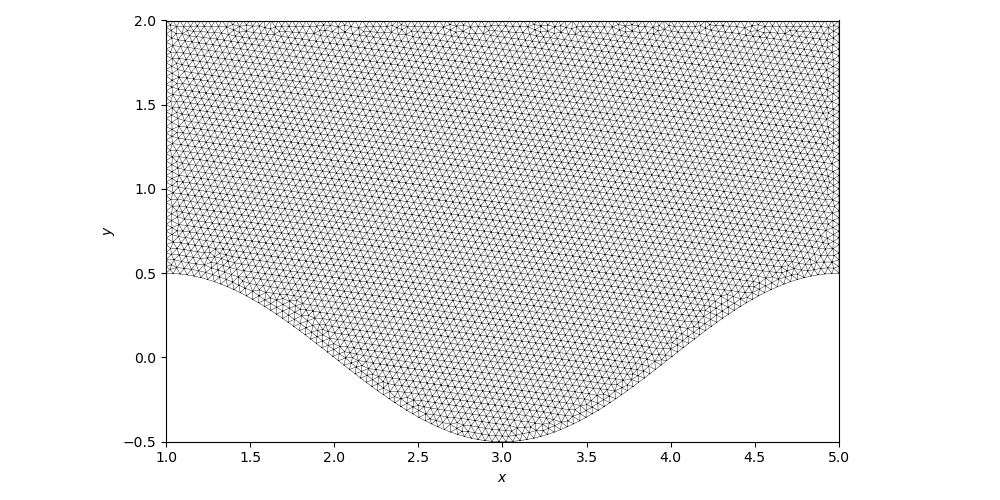
\includegraphics[width=1.5\columnwidth]{Test_domain_1_1_sin_mesh_0001_calfem_net_1.png}\\
							\hspace*{-18.5mm}
							\textit{a}
							
						\end{minipage}                                 
					} 
					{ 
						\begin{minipage}{0.47\textwidth} 
							\centering 
							\hspace*{-11.mm}
							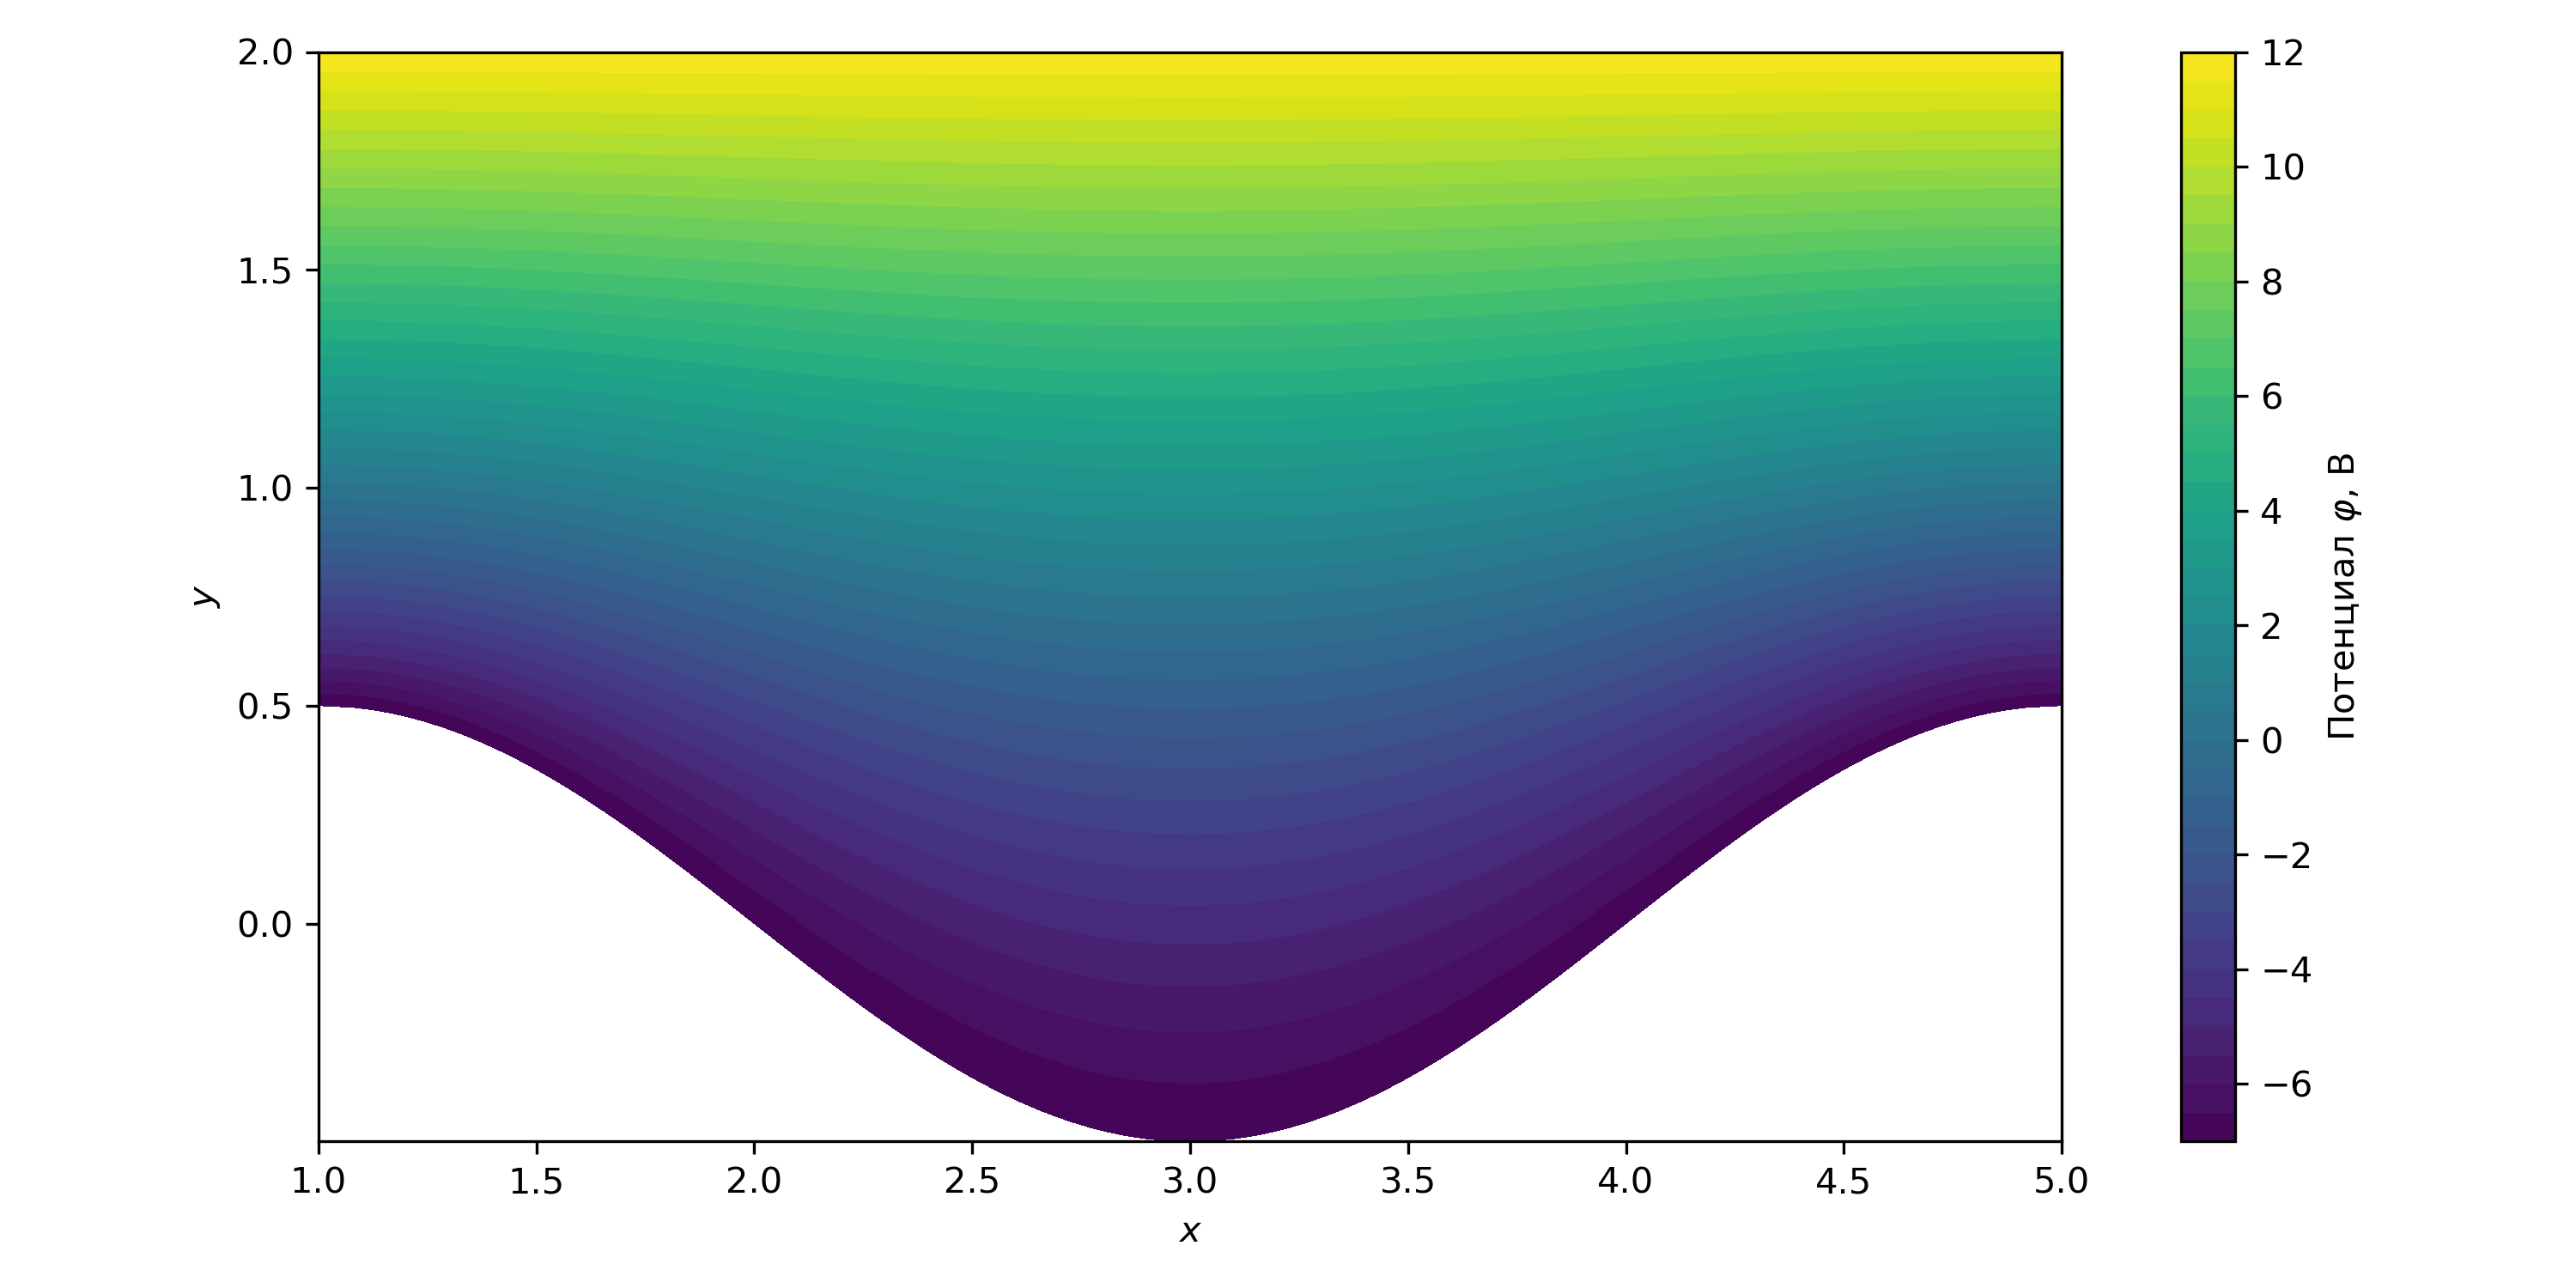
\includegraphics[width=1.5\columnwidth]{Test_domain_1_1_sin_mesh_0001_calfem.png}\\
							\hspace*{7.mm}
							\textit{b}						
						\end{minipage}                                 
					} 
					
				
				\vspace*{5mm}
				\caption{Иллюстрации к решению задачи №\,3 на отрезке $\left[ 1, 5 \right]$:\\
					\textit{a} --- иллюстрация разбиения исследуемой области с параметром $S_{max} \rightarrow 0.001$; \\
					\textit{b} --- численное решение задачи №\,3 с разбиением исследуемой области на  элементы с параметром $S_{max} \rightarrow 0.001$ \\
				} 
			\end{figure}
			
			Как и в задаче №\,2 расширим область до 3 периодов и рассмотрим точки, в которых значения решения должны совпадать.			
			
			\newpage
			
			\begin{figure}[h]       
				%\vspace{5.0mm} 
				\begin{center} 
					{ 
						\begin{minipage}{0.9\textwidth} 
							\centering 
							\hspace*{-25mm}
							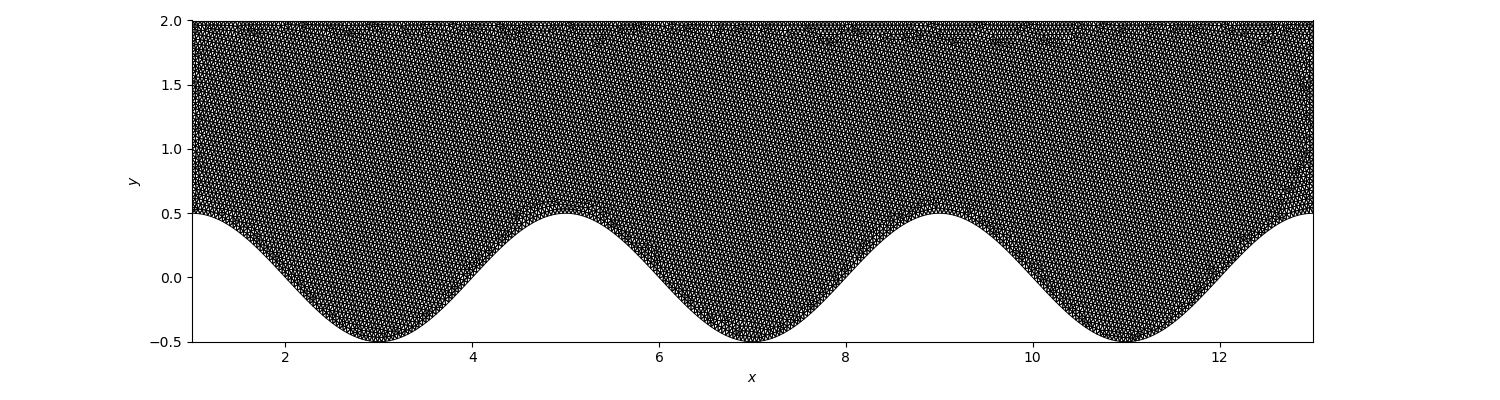
\includegraphics[width=1.35\columnwidth]{Test_domain_1_1_sin_mesh_0001_3_in_row_calfem_net_1.png}\\ 
							\textit{a} 
						\end{minipage}                                 
					} 
					{ 
						\begin{minipage}{1\textwidth} 
							\centering 
							\hspace*{-8.5mm}
							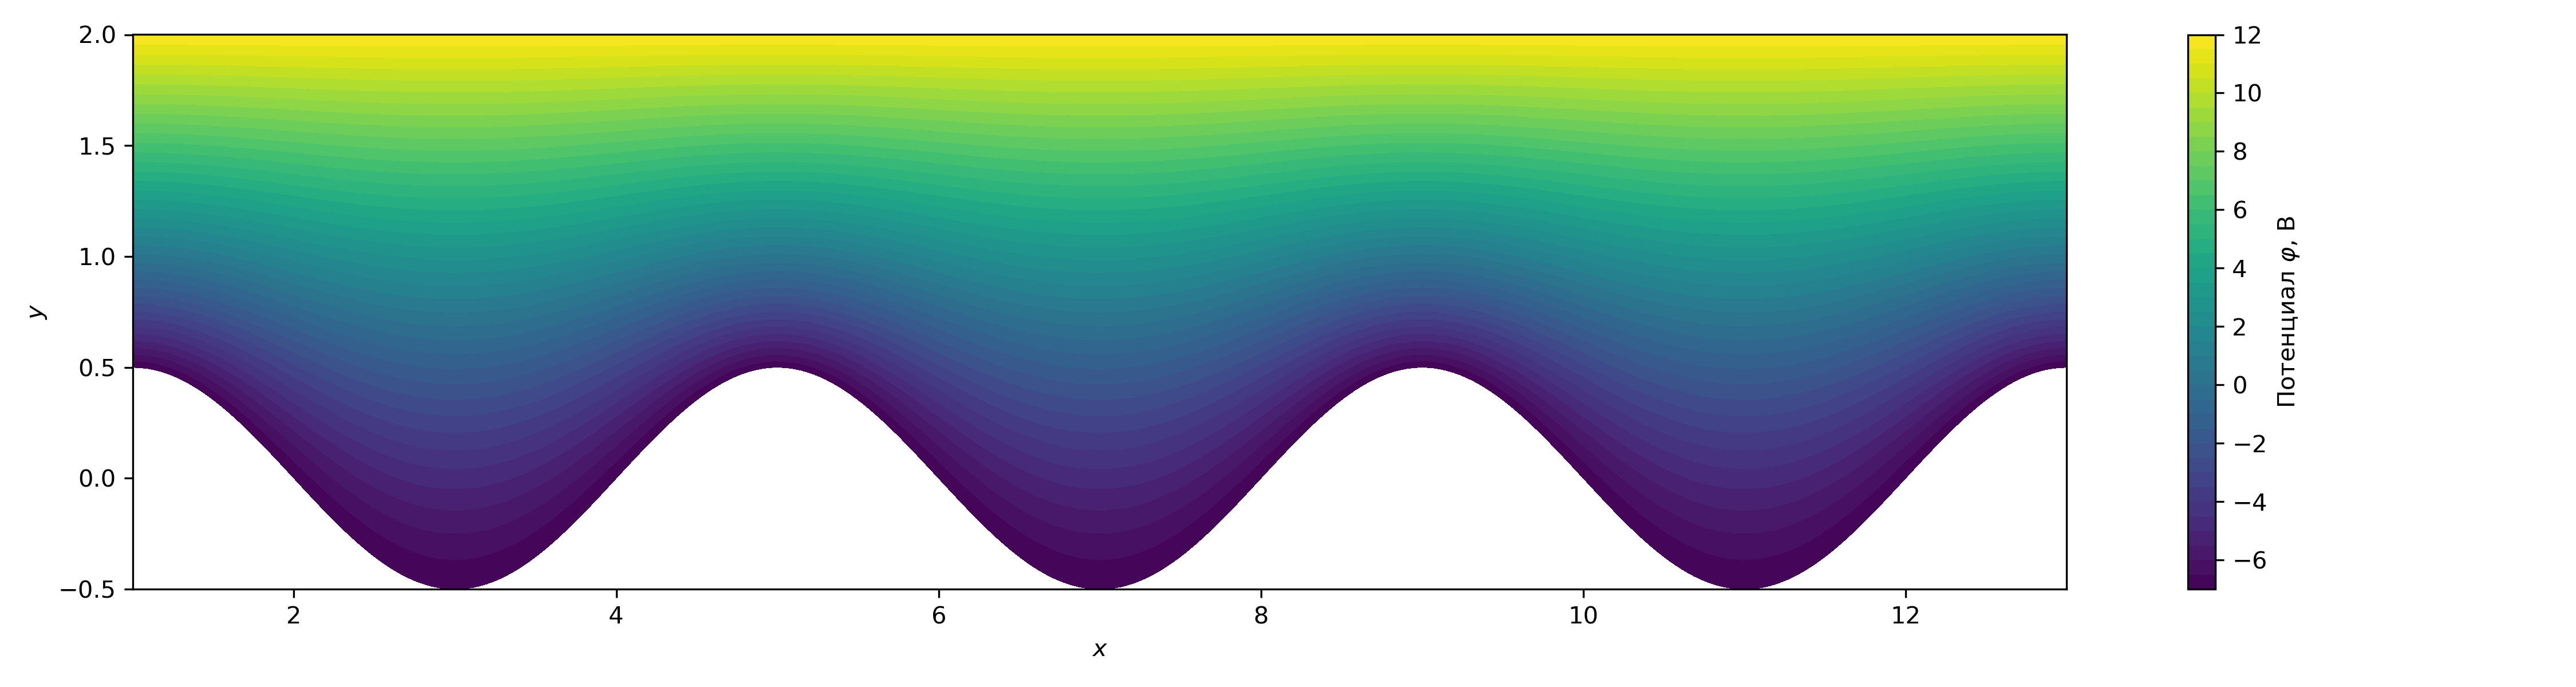
\includegraphics[width=1.2\columnwidth]{Test_domain_1_1_sin_mesh_0001_3_in_row_calfem.png}\\ 
							\textit{b} 
						\end{minipage}                                 
					} 
					
				\end{center} 
				\vspace*{-2.0mm} 
				\caption{Иллюстрации к решению задачи №\,3 на отрезке $\left[ 1, 13 \right]$:\\
					\textit{a} --- иллюстрация разбиения исследуемой области с параметром $S_{max} \rightarrow 0.001$; \\
					\textit{b} --- численное решение задачи №\,3 с разбиением исследуемой области на  элементы с параметром $S_{max} \rightarrow 0.001$ \\
				} 
			\end{figure}
		
		\subsubsection{Проверка решения на удовлетворение условиям периодичности}
			Аналогично предыдущей задаче проверим выполнение периодических граничных условий. Рассмотрим две группы точек:
			\begin{enumerate}
				
				\item Точки вида: $(1, y),\ (5, y)$ --- для решения построенного на одном периоде функции $w(x)$,
				$(1, y),\ (5, y),\ (9, y),\ (13, y)$ --- для решения построенного на трех периодах функции $w(x)$ (таблица \ref{table:comparison_sin_0001_1}).
				
				\item Точки вида $(1, y)$ --- для решения построенного на одном периоде функции $w(x)$,
				\looser{-0.02}{$(1, y),\ (3, y),\ (5, y)$ --- для решения построенного на трех периодах функции $w(x)$} (таблица \ref{table:comparison_sin_0001_2}).
				
			\end{enumerate}
			
			\newpage
			
			\begin{table}[!h]
				\centering
				\caption{ Сравнение\;значений\;численного\;решения\;задачи\;№\,3\;в\;первой\;группе\;точек 
				}
				\vspace*{2mm}
				\begin{NiceTabular}{|c|c|c|}[colortbl-like]
					\hline
					\rowcolor[HTML]{ededed} \xrowht{15pt}
					Область решения
					& Координаты $(x, y)$
					& Значение потенциала $\phi$, В\\ 
					
					\hline
					\hline
					
					\multirow{2}{*}{1 период $w(x)$}  
					& (1.0, 1.25)             
					& 3.4191          \\ 
					\cline{2-3} 
					
					& (5.0, 1.25)             
					& 3.4191          \\ 
					
					\hline
					
					\rowcolor[HTML]{ededed} \xrowht{5pt}
					\multirow{4}{*}{3 периода $w(x)$} 
					& (1.0, 1.25)             
					& 3.4191          \\ 
					\cline{2-3} 
					
					\rowcolor[HTML]{ededed} \xrowht{5pt}
					& (5.0, 1.25)             
					& 3.4185          \\ \cline{2-3} 
					
					\rowcolor[HTML]{ededed} \xrowht{5pt}
					& (9.0, 1.25)             
					& 3.4184          \\ \cline{2-3} 
					
					\rowcolor[HTML]{ededed} \xrowht{5pt}
					& (13.0, 1.25)            
					& 3.4191          \\ 
					
					\hline
					
					\multirow{2}{*}{1 период $w(x)$}  
					& (1.0, 1.6)            
					& 7.4927          \\ 
					\cline{2-3} 
					
					& (5.0, 1.6)             
					& 7.4927          \\ 
					\hline
					
					\rowcolor[HTML]{ededed} \xrowht{5pt}
					\multirow{4}{*}{3 периода $w(x)$} 
					& (1.0, 1.6)             
					& 7.4927          \\ 
					\cline{2-3} 
					
					\rowcolor[HTML]{ededed} \xrowht{5pt}
					& (5.0, 1.6)             
					& 7.4926          \\ 
					\cline{2-3} 
					
					\rowcolor[HTML]{ededed} \xrowht{5pt}
					& (9.0, 1.6)             
					& 7.4927          \\ 
					\cline{2-3} 
					
					\rowcolor[HTML]{ededed} \xrowht{5pt}
					& (13.0, 1.6)            
					& 7.4927        \\ 
					\hline
					
					
				\end{NiceTabular}
				\label{table:comparison_sin_0001_1}
			\end{table}
			
			
			
			
			\begin{table}[!h]
				\centering
				\caption{ Сравнение\;значений\;численного\;решения\;задачи\;№\,3\;во\;второй\;группе\;точек 
				}
				\vspace*{2mm}
				\begin{NiceTabular}{|c|c|c|}[colortbl-like]
					\hline
					
					\rowcolor[HTML]{ededed} \xrowht{15pt}
					Область решения
					& Координаты $(x, y)$
					& Значение потенциала $\phi$, В\\
					
					\hline
					\hline
					
					1 период $w(x)$                   
					& (3.0, 0.0)                                                       
					& -4.7379         \\ 
					\hline
					
					\rowcolor[HTML]{ededed} \xrowht{5pt}
					\multirow{3}{*}{3 периода $w(x)$} 
					& (3.0, 0.0)                                                       
					& -4.7382        \\ 					
					\cline{2-3} 
					
					\rowcolor[HTML]{ededed} \xrowht{5pt}
					& (7.0, 0.0)                                                       
					& -4.73749         \\ \cline{2-3} 
					
					\rowcolor[HTML]{ededed} \xrowht{5pt}
					& (11.0, 0.0)                                                      
					& -4.7386        \\ 
					
					\hline
					
					1 период $w(x)$                   
					& (3.0, 1.5)              
					& 7.205          \\ 
					\hline
					
					\rowcolor[HTML]{ededed} \xrowht{5pt}
					\multirow{3}{*}{3 периода$ w(x)$} 
					& (3.0, 1.5)              
					& 7.2051         \\ 
					\cline{2-3} 
					
					\rowcolor[HTML]{ededed} \xrowht{5pt}
					& (7.0, 1.5)              
					& 7.2051          \\ 
					\cline{2-3} 
					
					\rowcolor[HTML]{ededed} \xrowht{5pt}
					& (11.0, 1.5)             
					& 7.205          \\ 
					\hline
					
					
				\end{NiceTabular}
				\label{table:comparison_sin_0001_2}
			\end{table}



			Из таблиц \ref{table:comparison_sin_0001_1}, \ref{table:comparison_sin_0001_2} видно, что значения отличаются примерно на порядок $O(h^2)$, что показывает выполнение условий периодичности.
			
			
						
		
	
	\newpage
	\section{Программная реализация}
		
		Алгоритм для решения задачи методом конечных элементов (МКЭ) был реализован на языке C++. МКЭ предполагает решение системы линейных алгебраических уравнений с разреженной матрицей, для этого использовалась библиотека линейной алгебры для языка C++ --- Eigen \cite{eigen}. Для построения сеток использовались математический пакет Wolfram Mathematica и библиотека CALFEM \cite{calfem} для языка Python. Графики и иллюстрации строились с помощью встоенных средств Wolfram Mathematica и библиотеки Matplotlib \cite{matplotlib} для языка Python. 
		
	
	\section-{Заключение}
		
		В ходе курсовой работы был изучен и реализован метод конечных элементов для решения уравнения Лапласа. Реализация метода была проверена на тестовом примере с известным решением, также с ее помощью были решены и исследованы несколько вариантов исходной задачи с разными профилями пластин и заданными на них потенциалами.
		Все описанные подходы выполнены на языке C++ с демонстрацией результатов работы.		
	
	
	\newpage
	
	\begin{thebibliography}{4}
		
		\bibitem{Landau} Ландау Л.Д., Лифшиц Е.М. Теория поля. 6-е изд., испр. М.: Изд-во Наука, 1973. 507 с.
		
		\bibitem{Galanin} Галанин М.П., Савенков Е.Б. Методы численного анализа математических моделей. 2-е изд., испр. М.: Изд-во МГТУ им. Н.Э.~Баумана, 2018. 591 с.: ил. 
		
		\bibitem{Stahel} Stahel A. Calculus of Variations and Finite Elements. 2003. 
		URL:
		\href{https://www.researchgate.net/publication/268051850_Calculus_of_Variations_and_Finite_Elements}{https://www.researchgate.net/publication/268051850\_Calculus\_of\_Variations\_and} \href{https://www.researchgate.net/publication/268051850_Calculus_of_Variations_and_Finite_Elements}{\_Finite\_Elements} (дата обращения 27.05.2023)	
		%P. 151--152.
		\bibitem{calfem} CALFEM for Python. Computer Aided Learning of the Finite Element Method. 
		URL:  \href{https://calfem-for-python.readthedocs.io}{https://calfem-for-python.readthedocs.io/}
		(дата обращения 8.06.2023)	
		
		%\bibitem{wolfram} Wolfram Mathematica. The world's definitive system for modern technical computing \\
		%URL:  \href{https://www.wolfram.com/mathematica/}{https://www.wolfram.com/mathematica/} \\
		%(дата обращения 8.06.2023)	
		
		\bibitem{eigen} Eigen. C++ template library for linear algebra: matrices, vectors, numerical solvers, and related algorithms.
		URL:  \href{https://eigen.tuxfamily.org}{https://eigen.tuxfamily.org/}
		(дата обращения 20.05.2023)
					
		
		%\bibitem{python} Python.  A high-level, general-purpose programming language \\
		%URL:  \href{https://www.python.org/}{https://www.python.org/} \\
		%(дата обращения 20.05.2023)
		
		\bibitem{matplotlib} Matplotlib. A comprehensive library for creating static, animated, and interactive visualizations in Python. 
		URL:  \href{https://matplotlib.org/}{https://matplotlib.org/}
		(дата обращения 8.06.2023)
		
		
		
	\end{thebibliography}
	

\end{document}